\documentclass[UTF8,fontset=fandol,10pt,a4paper,openany]{ctexrep}
\usepackage[margin=22mm,headheight=15pt]{geometry}
\usepackage{amsmath,amssymb,booktabs,longtable,array,xcolor,hyperref,fancyhdr,enumitem,tikz}
\usetikzlibrary{arrows.meta,positioning}
\hypersetup{colorlinks=true,linkcolor=blue!45!black,urlcolor=blue!45!black}
\setlength{\parskip}{3pt}\setlength{\emergencystretch}{3em}
\setlist{nosep,leftmargin=2em}\raggedright\setlength{\parindent}{2em}
\pagestyle{fancy}\fancyhf{}\fancyhead[L]{20位SAR RTL：Dr. RTL方法的功能与时序分析}
\fancyhead[R]{2026-10-07}\fancyfoot[C]{\thepage}
\newcommand{\code}[1]{\nolinkurl{#1}}
\title{20位SAR ADC数字设计\\Dr. RTL方法下的功能、综合与时序分析}
\author{固定源码、generic综合与冻结布线检查点的独立交叉审查}
\date{2026年10月7日\\源基线：\code{01ed2b3e4fc4c7c9efd2153cfbfa5d456b10fb74}}
\begin{document}\maketitle
\begin{abstract}
本报告应用本机新安装的\code{asic-rtl-timing} skill，分析全部24个RTL模块及两个参数头。当前源码与同源历史功能见证字节一致，当前HEAD的10月2日CI九项已通过。本轮实际运行Yosys0.66对ADC2、MAC及divider P5/P7四项generic结构综合；并在远端Vivado2018.3重新打开SHA绑定的旧P5布线DCP导出setup/hold、扇出和约束。P7减少迭代但增加每拍结构工作量，核心最差路径77.875\%来自真实互连，权重库reset网扇出61236。25ns旧实现的核心setup/hold通过，外部OOC hold仍失败；不能据此宣称ASIC640MHz、完整模拟复现或全面PPA优势。本轮无生产RTL改写、无新综合布线循环、无本机STA安装，所有候选保留功能/等价、hold、面积与物理完成门控。
\end{abstract}\tableofcontents
\chapter{集成分析与实施判断}



日期：2026-10-07，Asia/Shanghai。源基线：\code{01ed2b3e4fc4c7c9efd2153cfbfa5d456b10fb74}。顶层：\code{sar20_digital_core}。本轮是分析任务，生产 RTL 保持原字节；不启动 RTL 优化循环，不晋级任何未证明的改写。


\section{结论与本轮新增证据}


当前设计已有多项有界、可追溯的数字验证，静态物理权重重构的数学与整数合同保持一致。当前最需要处理的是系数工作域、模拟接口的逐样本异常归属、物理 ID/权重选择的布线成本和实际时序验收条件。现有证据不能支持全参数无错误、论文电路全部复现、ASIC 640 MHz 达标或全面 PPA 优势。


本轮按本机 \code{asic-rtl-timing} skill 使用 Dr. RTL 的路径诊断和证据门控方法，分别完成源码功能复核、算术 cone 的实际 generic synthesis、历史布线检查点的真实远端重新导出，以及约束/候选改写审核。不是运行上游默认的 Nangate45/0.1 ns 商业流程，也没有执行 RTL-Timer 预测模型。


\begingroup\small\setlength{\tabcolsep}{2pt}\renewcommand{\arraystretch}{1.25}\begin{longtable}{@{}>{\raggedright\arraybackslash}p{0.25\linewidth}>{\raggedright\arraybackslash}p{0.32\linewidth}>{\raggedright\arraybackslash}p{0.39\linewidth}@{}}
\toprule
\textbf{证据} & \textbf{本轮实际完成} & \textbf{适用范围}\\\midrule\endhead
输入身份 & 24个生产SV、两个参数头SHA冻结；与10/02见证源字节全部相同 & 同源历史功能见证可追溯，不能称本轮重跑\\\addlinespace[2pt]
硬件来源桥 & 26份源与历史P5源包剔除注释/空白后词法tokens一致；源包成员SHA核验 & 有限语义来源桥，不是新综合或SEC\\\addlinespace[2pt]
当前CI记录 & 读取并封存对应当前HEAD的10/02 CI，9项全部SUCCESS & 含一项RTL job及软件/安装等检查；不是本轮重触发，不提供STA\\\addlinespace[2pt]
新结构综合 & Yosys0.66：ADC2、MAC、divider P5/P7，全部check通过 & generic原语、拓扑深度；没有Liberty面积或延迟\\\addlinespace[2pt]
新远端STA导出 & Vivado2018.3重开旧P5 routed DCP，setup/hold/扇出/约束重新导出 & 原器件、原25ns和原物理实现；不是当前默认P7新布线\\\addlinespace[2pt]
输入保持 & DCP分析前后SHA一致；无新综合、place/route、约束编辑 & 保证本轮报告来自同一冻结检查点\\\addlinespace[2pt]
\bottomrule\end{longtable}\endgroup


本机没有Verilator，定向RTL仿真在工具探测时退出1；原始命令与日志保留。缺工具不记作RTL失败，也不记作新PASS。实际功能动态依据为同源历史见证和当前HEAD的CI。用户既定“不在本机布置STA”边界得到保持：本轮真实STA导出在已有Windows Vivado上执行，没有安装STA。


本轮还取回该CI的原始RTL job与Python3.11日志：后者987 passed、3 deselected；RTL job含273条流程单测、P5/P6/P7各32样本的15/13/11T协议检查，以及独立算术审计MAC40010例、ADC40000例、divider10048例和8组flag序列。它们在10/02执行并绑定审查HEAD，不与本轮4个generic综合case或此前有界见证计数相加；通过不等于无限SEC或模拟性能验证。


CI实际checkout是PR自动合并提交 \code{86499bbfa99c942a319c398151335648cdd4b114}，不是分支提交本身。已核对Git树：它与审查HEAD仅README不同，26个RTL/头文件以及软件、测试、工具和流程文件全部相同；完整关系保存在 \code{baseline/ci_tree_binding.json}。不能只凭PR绿标声称测试了某份源字节。


\section{固定条件：三个对象必须分别评价}


当前生产源默认 \code{P_STRUCTURAL=1}、\code{P_RECON_STAGES=7}、ADC2=12 bit、输出20 bit、18 slice、每笔8 active、每slice 63 main+8 sub、16相位帧、权重Q30、电压Q32。比较器与配置输入必须与 \code{clk} 同步；所有生产时序状态使用同步低有效reset。


真实硬件报告属于P5，Virtex-7 \code{xc7vx690tffg1761-2}，Vivado2018.3，OOC，25.000ns，内部BUFG，0.05ns用户uncertainty，零I/O min/max。报告包含工具的Slow/Fast delay corner分析；这不是ASIC的PVT/MMMC覆盖。路径实际uncertainty为0.085ns，不能只取用户设置0.05ns来重算slack。


ASIC目标是640MHz、时钟周期1.5625ns、16拍对应40MS/s。该目标必须用项目实际Liberty、宏模型、模式/角、SDC、时钟与寄生验证。目前缺这些输入，因此本轮不输出ASIC WNS/TNS、面积、功耗或Fmax估计。


\begingroup\small\setlength{\tabcolsep}{2pt}\renewcommand{\arraystretch}{1.25}\begin{longtable}{@{}>{\raggedright\arraybackslash}p{0.19\linewidth}>{\raggedright\arraybackslash}p{0.24\linewidth}>{\raggedright\arraybackslash}p{0.27\linewidth}>{\raggedright\arraybackslash}p{0.26\linewidth}@{}}
\toprule
\textbf{条件} & \textbf{当前RTL功能} & \textbf{旧P5物理实现重开} & \textbf{ASIC目标}\\\midrule\endhead
divider展开数 & 默认P7；P5是可选合同 & P5 & 必须固定后重建基线\\\addlinespace[2pt]
工艺/器件 & 与工艺无关的RTL语义 & Virtex-7 -2 & 项目认可Liberty/PVT待提供\\\addlinespace[2pt]
时钟与帧 & 16拍；P7重构11T，P5为15T & 25ns；每帧400ns，2.5MS/s & 1.5625ns；每帧25ns，40MS/s\\\addlinespace[2pt]
数字功能证据 & 当前CI及同源历史RTL见证 & 旧完整映射功能见证另有身份 & 需目标网表对应验证\\\addlinespace[2pt]
物理证据 & 无当前P7新物理结果 & 新导出同一个旧routed DCP & 尚未测量\\\addlinespace[2pt]
\bottomrule\end{longtable}\endgroup


\section{设计功能与校准算法}


结构核实现共享3-bit Flash、双9-bit粗SAR、12-bit fine SAR、18-slice因果轮换、二维DEM、dither、RDAC已决码更新、残差上下文冻结、物理权重修正、输出ID/flags和配置状态。兼容模式接受外部现成coarse/fine码，是不同的elaboration profile，不能用它的通过替代逐位结构模式。


校准系数训练在片外，片上装载并应用系数；没有片上LMS/RLS自学习引擎。物理权重包含电容反馈比例、bridge衰减和约定有效增益，不能在重构后再次无条件乘除32。


\[F=O+Gx+R+TI,\quad T=\sum w,\quad G=\sum wa,\quad R=T-2\sum w_{on}+\sum w_r.\]


\[x=(F-O-R-TI)/G.\]


RTL按真实物理ID和已发生的DEM/RDAC/采样状态计算T/G/R，并冻结前一残差的上下文。sampling dither单元从G扣除，但其电荷仍计入T/R。这一模型依赖线性、稳定和一致的参数；真实RA非线性、记忆、参考建立和输入相关注入需要模拟模型与测量。


整数数据通路先用扩位乘加检查96-bit合同，再保留117-bit shifted，取63-bit signed numerator交给正unsigned gain的floor divider。负且非整除的结果必须向负无穷下修，不能替换为向零截断；输出先作signed边界判断再饱和成20-bit offset-binary。


\subsection{数值合同尚需工程化的部分}


ADC2实现 \code{min + RTE(delta)}，而不是对绝对中心整体RTE。min为奇数且增量恰为半整数时可差1个Q32整数LSB。此语义与冻结oracle一致，不是默认RTL/oracle mismatch；任何修改必须同步升级合同、软件和RTL。


\code{cfg_ready}证明系数装载完整和配置字段合法，不证明所有系数在全输入范围下都满足MAC工作域。例如中点需要G\_Q严格小于2\textasciicircum{}43，归一化x=+1需要严格小于2\textasciicircum{}42；正常名义G\_Q=32\ensuremath{\times}2\textasciicircum{}30安全，但每个单元合法并不自动保证组合的全量程安全。训练/装载软件必须使用机器可检验的工作域，RTL应按明确异常合同报告超界。


\code{cal_weight_reduce}的缓存行和必须与同一份权重同时更新。顶层已同源连接；单独复用该模块的集成者不能提供陈旧row totals。算术压位需要证明对整个合法域保持overflow、rounding、floor和clamp，而不是只证明标称正弦数据一致。


\subsection{控制和异常合同}


粗SAR固定Flash seed的高3位，只搜索低6位。跨64码桶的seed错误无法由低位搜索纠正；popcount不检测bubble。应给Flash seed误差、valid和建立时间明确宏合同，再做offset/bubble/迟到故障扫描。


缺比较器valid可暂停位判决，但16相位帧不延长；到deadline仍取消并drop。因此比较器建立时间与传回valid延迟直接决定实际吞吐，不能从计数器周期推出模拟转换成功。


模拟bad在规定transfer/quiet边沿采样；取消、过期或被后包替换的fault是否sticky、是否逐样本可见必须明确。当前5-bit \code{dout_flags}没有独立analog\_bad位，sticky状态不等同逐样本fault归属。数值acc/gain异常保留上个合法码，软件必须同时读valid、ID、flags。


默认dither D=2下valid恒1；某些非默认D需要rejection重抽，调用点未统一为同一样本重抽。默认不触发，但不能宣称所有可声明参数都已验证。论文的双dither、跨ADC tracking、ADC2宽窄带切换和模拟AUX/RA/reference等结构仍有既有边界，详见10/02报告及本轮功能附录。


\section{当前算术cone的真实generic synthesis}


采用已安装Pyosys入口，Yosys0.66，git sha \code{86f2ddebc}。每项都读取真实源/头文件，执行 \code{hierarchy -check}、\code{proc/opt/check -assert}、\code{synth -noabc}、再次 \code{check -assert}；保留精确命令、日志、pre JSON及generic JSON/Verilog。没有删掉不支持语言结构，没有引入替代ASIC库。


\begingroup\small\setlength{\tabcolsep}{2pt}\renewcommand{\arraystretch}{1.25}\begin{longtable}{@{}>{\raggedright\arraybackslash}p{0.2\linewidth}>{\raggedright\arraybackslash}p{0.15\linewidth}>{\raggedright\arraybackslash}p{0.17\linewidth}>{\raggedright\arraybackslash}p{0.16\linewidth}>{\raggedright\arraybackslash}p{0.28\linewidth}@{}}
\toprule
\textbf{Cone} & \textbf{generic组合原语} & \textbf{状态bit} & \textbf{最长拓扑深度} & \textbf{说明}\\\midrule\endhead
ADC2 decoder & 6533 & 0 & fine\_q=81；ovf=80 & 含range subtraction、乘法、舍入/比较/clamp\\\addlinespace[2pt]
residue MAC & 29157 & 0 & a1=78；any\_ovf=95 & 含扩位乘减和受检工作域；异常锥不能删掉\\\addlinespace[2pt]
divider P5 & 3862 & 317 & 状态D=140 & 5级串接borrow/sub/mux；13次迭代\\\addlinespace[2pt]
divider P7 & 4917 & 313 & 状态D=184 & 7级串接borrow/sub/mux；9次迭代\\\addlinespace[2pt]
\bottomrule\end{longtable}\endgroup


这些计数是同一generic流程下的单bit原语统计；不是LUT、标准单元面积或时延。拓扑深度以输入/FF Q为0，每个组合原语算一级；FF D/E/R分别统计，时钟不算数据路径。全部四项没有latch、memory、未解析bit或残余内部算术cell。


P7相对P5的generic组合原语增加27.3\%，最大D拓扑深度增加31.4\%，FF少4。原因是P5把幅值/商pad到65位，P7为63位；更多除法步在同一拍展开。这个结构结果说明吞吐/延迟与每拍工作量的权衡，不能据此断言某工艺的P7更慢31.4\%。


divider已经用一次扩位subtract同时形成borrow和余数决策，不存在独立全宽compare再重复subtract。最长结构路径还包含负数floor修正、余数非零判断、商加一/取负和最终提交选择。按Dr. RTL诊断，优先定位真实divider路径的这一尾端，再考虑算术结构；不能只把源码循环拆开或随意删符号修正。


ADC2有13个独立数据位乘65-bit range表达；frontend端口缩减后显示14\ensuremath{\times}65，其中多1bit是常量保护位。MAC有64\ensuremath{\times}64数据变量，frontend表达为65\ensuremath{\times}64保护形式。宽声明或中间\$mul名字不代表同宽独立物理乘法器，更不能作为ASIC单元面积。


\section{完整核的存储、归约和选择成本}


权重库的数据bit为18\ensuremath{\times}71\ensuremath{\times}47=60066；loaded bitmap1278；18行54-bit缓存972；合计62316候选状态bit。历史实测权重库FF为62316、全核FF为66492，比例93.72\%。完整核历史综合为108842 LUT、66492 FF、20 DSP、0 BRAM、0 latch；这属于旧P5综合，不能转写成当前ASIC面积。


权重按物理单元并行被归约读取。on-tree有1278叶子、补齐2048叶子、11层拓扑；row cache只去掉total-tree，不去掉on-tree。ID匹配、重复检查和物理mask散射同时造成大量逻辑关系。单端口RAM无法在一拍交出同样读数；只加 \code{ram_style} 不会保持现有接口和周期合同。


简单串行单端口读568个所需物理权重需要568次访问；18个单端口bank逐行读71次。这只是朴素方案的计数，不是所有RAM架构的不可突破下界。真正的存储优化需要先从样本捕获窗、物理ID和开关规则导出足够的分组/预归约/缓存，再证明所有事务的结果与时序合同。


面积目标应按数据系数、row cache、选择/归约、MAC、divider、控制分别分解。FPGA rebuilt层级可能移动归属，不能把parent+child资源重复相加。没有活动注入，功耗缺真实SAIF/VCD和宏功耗模型，本轮不报功耗优势。


\section{新导出的真实布线STA与路径}


远端主机别名 \code{windows-codex}，机器REEDZHAO，Vivado2018.3。输入是原P5布线DCP，SHA \code{fba86312b0c96add78ca388b972a52ab77c1b781eec34c1b91027b1ea7358072}。只执行 \code{open_checkpoint} 和报告/约束导出；没有综合、placement、route或例外/时钟编辑。执行记录证明输入前后SHA相同，原始路径与本轮指标一致。


\begingroup\small\setlength{\tabcolsep}{2pt}\renewcommand{\arraystretch}{1.25}\begin{longtable}{@{}>{\raggedright\arraybackslash}p{0.19\linewidth}>{\raggedright\arraybackslash}p{0.24\linewidth}>{\raggedright\arraybackslash}p{0.27\linewidth}>{\raggedright\arraybackslash}p{0.26\linewidth}@{}}
\toprule
\textbf{检查范围} & \textbf{setup WNS} & \textbf{hold WHS} & \textbf{结论}\\\midrule\endhead
全部OOC路径 & +0.946ns，TNS=0 & -2.278ns，\code{THS=-110433.469ns} & 65048个hold failing endpoints，整体未闭合\\\addlinespace[2pt]
register clock\ensuremath{\rightarrow}register data & +0.946ns & +0.052ns & 该范围25ns setup/hold满足；不是完整外部接口\\\addlinespace[2pt]
脉宽 & WPWS=12.100ns & TPWS=0 & 对应该时钟/器件检查\\\addlinespace[2pt]
\bottomrule\end{longtable}\endgroup


最大核心路径为 \code{u_structure/u_context/fine_slices_reg[1][3]/C} 到 \code{u_recon/rails_s_reg[65]/D}，\code{requirement25.000ns}，data23.914ns，其中cell5.291ns、route18.623ns，40个器件逻辑level，route占77.875\%。它连接物理slice选择到权重/rail归约快照；应优先审查ID解码扇出、权重阵列布局和归约布线。单纯优化一个加法表达式很难解释这里主要的18.623ns连线。


最小核心路径为 \code{residue_reg[570]/C} 到 \code{fine_main_reg[6][59]/D}，data0.263ns，cell0.118ns、route0.145ns，0个器件逻辑level，hold +0.052ns。这里0 logic levels不等于0 cell delay，FF clock-to-Q仍计入路径。默认phase9 residue\_capture到下一phase0 quiet\_sample约7T，属于另一组精确transfer MCP候选；仍需证明\code{clear/disable/first-frame}、capture和下一次改动，并配对hold，不能直接设置7T例外。


最差全接口hold为 \code{cfg_wdata[3]} 到 \code{u_wstore/w_q_reg[13][36][3]/D}，slack -2.278ns。当前零I/O min假设配合OOC外部时钟边界，不能保证外部最早到达与内部capture时钟的关系。不能删除该路径、凭空加输入min或全局false path来宣称通过；必须取得真实发送端clock-to-out、封装/走线/宏相位和接收端预算，再按真实条件实现并验收。


实际时钟端点有66508个clock pins，D/E/R数据集合199440个pins；这个过滤统计与66492个FF资源不是同一对象，不能要求两数相等。大集合触发工具性能warning，报告已完成；不把性能提示当时序违规或忽略部分端点。


\section{新的高扇出实测：控制和配置也有物理成本}


\begingroup\small\setlength{\tabcolsep}{2pt}\renewcommand{\arraystretch}{1.25}\begin{longtable}{@{}>{\raggedright\arraybackslash}p{0.19\linewidth}>{\raggedright\arraybackslash}p{0.24\linewidth}>{\raggedright\arraybackslash}p{0.27\linewidth}>{\raggedright\arraybackslash}p{0.26\linewidth}@{}}
\toprule
\textbf{routed net} & \textbf{fanout} & \textbf{驱动类型} & \textbf{优化关注}\\\midrule\endhead
u\_wstore/SR[0] & 61236 & LUT1 & 权重库同步复位控制的全局负载\\\addlinespace[2pt]
u\_wstore/u\_idx[2] & 6776 & LUT6 & 权重写单元译码跨大量bank负载\\\addlinespace[2pt]
u\_calib/phase0 & 1864 & LUT2 & 配置阶段/共同条件扇出\\\addlinespace[2pt]
\code{u_structure/u_phase/phase_reg}[3]\_2[0] & 1369 & LUT5 & frame相位控制负载\\\addlinespace[2pt]
\code{u_calib/cfg_ready_reg_4}[0] & 1368 & LUT2 & epoch/enable控制负载\\\addlinespace[2pt]
cfg\_wdata[46] & 1322 & PORT & 配置输入物理分发\\\addlinespace[2pt]
其余多条cfg\_wdata & 1321 & PORT & 同类配置路径，含最差hold源\\\addlinespace[2pt]
\bottomrule\end{longtable}\endgroup


fanout数量不是延迟，最高fanout网也不一定出现在最差数据路径。它提供了配置/复位域物理规划的新证据：可以评估局部译码、布局区域与物理buffer/复制；需要检查实际arrival、slew/cap和拥塞后决定。


不能直接取消权重reset：当前reset后的配置读回、未载入数据、row total和bitmap具有确定合同。若改为只reset metadata，必须定义未载入读回及写入增量更新语义，并同时验证软件、formal与映射；这属于具体候选架构变化，不是本轮已执行的优化。


\section{SDC/XDC审查与多周期边界}


新导出的exception报告显示false path、clock groups、multicycle、max/min delay六类计数全部0。当前真实STA使用一拍约束，没有通过例外掩盖关键路径；zero uncovered categories只说明在所记录OOC假设下约束覆盖，并不证明预算来自真实外部电路。


样本context在pre-phase0更新，重构Stage-A在pre-phase15接受，相隔15T；fine code在pre-phase14更新，仍只有1T。16相位帧不是整个核的16周期例外。只有源稳定性、最早捕获、下一次改动、\code{clear/enable/cancel}、权重epoch、ID同行和具体网表端点都证明后，才可评估精确MCP。setup和hold移动关系需要同时检查，不能只设置setup。


目前有限wrapper有57笔接受的15T/1T证据，但不含真实完整归约通路，也不是全序列形式证明，未覆盖全配置clear/re-enable。该证据提供候选依据，不足以立即套例外。本轮没有增加任何MCP或false path。


同步reset作为普通同域数据控制检查；没有异步reset recovery/removal问题的同等证据义务。若后续顶层输入成为异步reset/比较器/配置域，则必须另外引入同步/CDC合同与相应物理检查，不能把当前接口默认当已跨域安全。


\section{Dr. RTL策略如何具体应用到本设计}


\begingroup\small\setlength{\tabcolsep}{2pt}\renewcommand{\arraystretch}{1.25}\begin{longtable}{@{}>{\raggedright\arraybackslash}p{0.19\linewidth}>{\raggedright\arraybackslash}p{0.24\linewidth}>{\raggedright\arraybackslash}p{0.27\linewidth}>{\raggedright\arraybackslash}p{0.26\linewidth}@{}}
\toprule
\textbf{真实瓶颈/证据} & \textbf{策略类别} & \textbf{可评估候选} & \textbf{必须保持/证明}\\\midrule\endhead
context ID\ensuremath{\rightarrow}rails，77.875\% route & fanout/local decode；策略7/8/21 & 物理分区、局部ID谓词、控制复制、缩短权重到归约距离 & 同沿ID/DEM/采样/RDAC一致；reset/使能优先级；复制未被综合合并；实际route收益\\\addlinespace[2pt]
weight reset61236、unit index6776 & 高扇出控制，策略7/8 & 局部译码与工具物理buffer；评估metadata reset候选 & 原\code{reset/readback/cache}合同；不能增加未批准延迟；面积/hold/拥塞\\\addlinespace[2pt]
divider串接borrow及floor尾端 & arithmetic策略9/10；宽度策略28 & 真实carry/borrow结构优化，分组数P5/P6/P7同条件比较 & signed最小值、负非整除、zero/large gain、padding、\code{start/cancel/latency}\\\addlinespace[2pt]
MAC any\_ovf最长generic锥 & width明确化策略28 & 先证明系数域，再分别评估数据和overflow计算 & 异常可见性、超界分类、符号/截断/舍入；不得删除检查取得快路径\\\addlinespace[2pt]
62kFF系数存储 & 结构架构评估 & 分组/预归约/多bank与时间窗计划 & 等价读数、所有物理组合、配置epoch、16拍和事务ID\\\addlinespace[2pt]
context 15T、fine code1T & 约束证明，先于RTL改写 & 精确MCP形式不变量及端点清单 & 稳定/捕获/next-change；配对hold；无wildcard blanket exception\\\addlinespace[2pt]
\bottomrule\end{longtable}\endgroup


共享谓词/CSE并非一定更好：route主导时，全局共享可能增加负载。局部复制也可能被综合重新合并、增加状态/面积或恶化拥塞。Dr. RTL“高置信度”是经验分类，必须通过真实工具，而不是把源文件换写法算优化成功。


禁止未经证明压窄系数或乘加器、重排有符号溢出运算、去掉floor修正、强迫已有平衡树变成自定义mux，或新增流水级却沿用旧ID/valid。低功耗也需要真实样本活动/clock enable和芯片宏功耗证据，不能仅从generic gates推出。


\section{已有候选为何不能晋级}


旧P7 640MHz OOC实验同时改了reducer与divider，LUT171246\ensuremath{\rightarrow}199039（+16.23\%），setup WNS -17.426\ensuremath{\rightarrow}-17.112ns（+0.314ns），hold TNS反而恶化0.528ns。它是旧输入、估计互连且联合改动，不能归因单模块；没有全面PPA优势或640MHz闭合。


旧local-row P5候选综合完成，但布线出现level-7 congestion，route\_design失败。中途+2.114ns不是最终STA，不能晋级。用更多局部树/复制可能增加布线压力，候选必须重建同条件基线并保留失败证据。


本轮未产生RTL候选，因此skill的 \code{compare_runs.py} 不构造伪造的ASICLiberty/area输入，也不把FPGA LUT填到area\_um2。该助手用于真实同条件ASIC STA候选门控；它本身不执行STA/SEC，不认证日志。后续实际优化才填写\code{baseline/candidate}，等价unknown、未约束、hold恶化、面积超预算或route未完成均不得晋级。


\section{下一轮实施的里程碑与验收}


\subsection{先完成可机器判断的功能与接口边界}


固定配置epoch、系数可用域、模拟error的有效边沿/样本归属、Flash seed允许误差、dither参数支持域，以及\code{structural/legacy} profile。当前功能回归与有限见证应保留独立整数真值、边界和fault ID检查。明确cfg-clear丢弃在途、busy start不接受、COMMIT可接下一start、\code{first-valid/re-enable}的行为。


只进行一个具体改动的候选；端口/复位/使能/优先级/latency保持不变时建立对应SEC。形式假设包括同步输入、合法epoch和真实宏deadline；不得把async2sync抽象或有限仿真说成所有reset行为的无限等价。需要改流水/握手时先给出完整新周期与ID合同。


\subsection{为真实ASIC STA补齐输入}


锁定实际顶层/参数、Liberty各角与单位、标准单元/存储/analog macro timing、SDC、合法模式、640MHz目标与I/O min/max/负载/驱动来源。综合/elaboration检查black box、未解析/残余generic cell、latch/loop与面积；有意宏不能靠black box默认忽略延迟。


在真实链接网表加载约束，核对集合数量、有效边沿、uncertainty、latency、IO及例外覆盖。setup/max与hold/min、transition/cap、pulse/gating和适用reset检查分别保存WNS/TNS及完整路径；没有数据的指标写未测量。


\subsection{物理实现与候选晋级}


按slice/weight/归约的连通关系规划placement，避免大总线跨全核；先检查高扇出与布局拥塞，再优化算术。CTS后用实际时钟检查hold，route后用对应寄生复核setup/hold与注入覆盖、DRC、拥塞和route完整性。活动标注功耗与面积/时序一起比较。


\code{baseline/candidate}保持相同参数、库、角、SDC、工具选项及物理条件。记录原生单位差值，不用WNS百分比，也不倒数一条数据延迟称Fmax。只有必要回归/SEC通过、setup改善、hold不恶化、面积在明确预算内且route完成的候选可以晋级；未闭合仍保持未闭合标签。


\section{交付、原始证据与复算方式}


主报告、功能/约束/结构附录、命令、SHA、generic网表和新导出的Vivado报告一起封存。\code{baseline/source_identity.json}连接当前源、历史功能和P5来源桥；\code{baseline/github_pr_ci.json}是本轮读取的当前CI状态。\code{baseline/reopened_route/execution.json}记录DCP前后SHA；\code{baseline/reopened_route/out/}保留\code{max/min/core/exception/clock/fanout/constraints}。


\code{cone_synthesis/}包含真实Yosys命令、4项日志和网表；其统计可以仅解析已有JSON重新计算，仍不生成STA。原执行cwd和之后搬移路径注明，不能把搬移后相对输出地址冒充原始工具入口。


正式PDF使用同目录独立LaTeX源和内嵌矢量图，按用户 \code{latex-macos-report-compile} 工作流导出，同时使用内置LaTeX编辑器编译核验。原始论文/专利没有重新发布；本轮是对现存RTL及已核对原理的Dr. RTL工程评价，不声称重新逐页重审16份原文。


官方约束依据：\href{https://docs.amd.com/v/u/2018.3-English/ug903-vivado-using-constraints}{AMD UG903 v2018.3}，Chapter4 I/O delay与Chapter5 timing exceptions。实际命令能力以本轮Vivado2018.3 \code{help report_high_fanout_nets}和完整日志为准，不把当前2026.1网页选项无条件套到旧版本。
\chapter{原创图与证据边界}
以下图均来自本轮实际工具报告。前两图属于旧P5 routed FPGA检查点的本轮重新导出；第三图属于当前源的generic结构综合。它们不是模拟波形、ASIC面积/功耗预测或新布局实现。
\section{实际核心路径及全接口hold}
\begin{center}\begin{tikzpicture}[x=.43cm,y=1cm]
\fill[blue!70] (0,0) rectangle (5.291,.75);
\fill[orange!75] (5.291,0) rectangle (23.914,.75);
\draw[red!65!black,dashed,thick] (25,-.2)--(25,1.2);
\node[text=white] at (2.6455,.375) {5.291};
\node at (14.6025,.375) {18.623 ns};
\node[above] at (12,.85) {cell 22.125\%；route 77.875\%};
\draw[->] (0,-.2)--(27,-.2);
\foreach \v in {0,5,10,15,20,25}{\draw (\v,-.2)--(\v,-.35) node[below]{\small\v};}
\node[align=left,anchor=north west] at (0,-1.1) {data=23.914 ns；时钟requirement=25.000 ns\\实际setup slack=+0.946 ns，包含clock/skew/uncertainty};
\end{tikzpicture}\end{center}
\begin{center}\begin{tabular}{lrr}\toprule 范围&Setup(ns)&Hold(ns)\\\midrule 核心寄存器路径&+0.946&+0.052\\全OOC路径&+0.946&\textcolor{red!70!black}{-2.278}\\\bottomrule\end{tabular}\end{center}
最差setup是\code{fine_slices_reg[1][3]}到\code{rails_s_reg[65]}。最差外部hold源是\code{cfg_wdata[3]}。图中的25ns虚线只是时钟周期；不能用25减23.914代替实际slack计算，也不能倒数data delay报告Fmax。
\section{高扇出网的新实测}
\begin{center}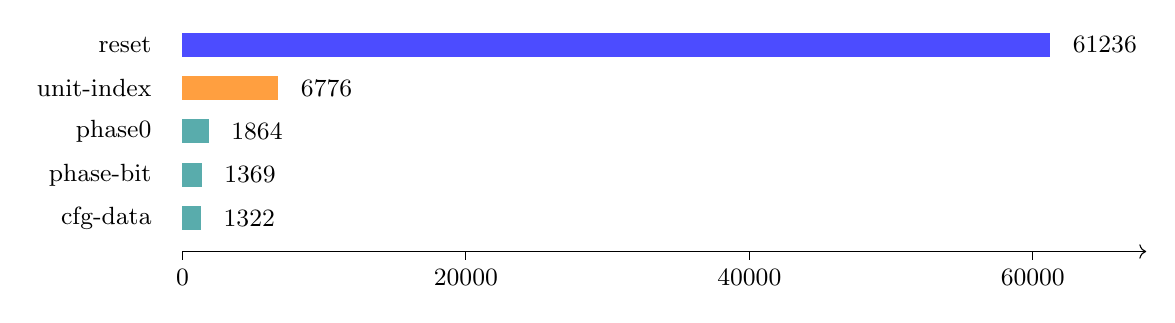
\begin{tikzpicture}[x=.18cm,y=.55cm]
\fill[blue!70] (0,4) rectangle (61.236,4.55);
\fill[orange!75] (0,3) rectangle (6.776,3.55);
\fill[teal!65] (0,2) rectangle (1.864,2.55);
\fill[teal!65] (0,1) rectangle (1.369,1.55);
\fill[teal!65] (0,0) rectangle (1.322,.55);
\foreach \y/\pos/\n/\label in {4/61.236/61236/reset,3/6.776/6776/unit-index,2/1.864/1864/phase0,1/1.369/1369/phase-bit,0/1.322/1322/cfg-data}{\node[anchor=east] at (-1.5,\y+.27) {\small\label};\node[anchor=west] at (\pos+.9,\y+.27){\small\n};}
\draw[->] (0,-.5)--(68,-.5);
\foreach \pos/\label in {0/0,20/20000,40/40000,60/60000}{\draw (\pos,-.5)--(\pos,-.7) node[below]{\small\label};}
\end{tikzpicture}\end{center}
数据来自\code{report_high_fanout_nets}。fanout表示负载数量，不是路径延迟；最高负载并不必然等于最差数据路径。该图解释权重库reset/配置/解码分发为何需物理规划，不证明取消reset或强制复制就会改善。
\section{P5/P7的结构与周期权衡}
\begin{center}\begin{tabular}{lrr}\toprule generic流程指标&P5&P7\\\midrule 组合原语&3862&4917\\单bit FF&317&313\\最长状态D拓扑深度&140&184\\迭代次数&13&9\\重构合同延迟(T)&15&11\\\bottomrule\end{tabular}\end{center}
\begin{center}\begin{tikzpicture}[x=.05cm,y=.9cm]
\fill[blue!70] (0,1) rectangle (140,1.6);\fill[orange!75] (0,0) rectangle (184,.6);
\node[anchor=east] at (-3,1.3) {P5};\node[anchor=east] at (-3,.3) {P7};
\node[text=white] at (70,1.3) {140};\node at (92,.3) {184};
\draw[->] (0,-.3)--(205,-.3);\foreach \x in {0,50,100,150,200}{\draw (\x,-.3)--(\x,-.45) node[below]{\small\x};}
\node[anchor=north west] at (0,-1) {最长D拓扑深度；不含cell/wire时延模型};
\end{tikzpicture}\end{center}
同一generic流程里，P7组合原语增加27.3\%、最大D深度增加31.4\%，但迭代减少4拍。不能称为同百分比的真实时延恶化；P5/P7的物理比较还需固定真实实现条件和功能合同。
\appendix

\chapter{24模块的功能复核与样本合同}


\section{范围与判断}


本次按本机 \code{asic-rtl-timing} skill 的“先确认源清单与功能边界、再区分 RTL 合同和实现证据”方式审查。目标仓库是 \code{outputs/sar_adc_review_20260919/calibration-closure}，当前 HEAD \code{01ed2b3e4fc4c7c9efd2153cfbfa5d456b10fb74}，工作树干净。以 \code{rtl/rtl_sources.f} 为入口检查全部 24 个生产 SystemVerilog 文件和两个参数头文件，并重点复核顶层、控制器、权重装载、校准归约、ADC2 解码、MAC、floor 除法及结果提交。


\textbf{本轮没有发现新的、已确认的默认配置功能错误。} 这不是全参数形式证明，也不是本轮重新跑过的 RTL 仿真、综合、STA 或模拟验证。现有算术/控制结论中，有几项是此前已有记录；本报告将其作为待遵守边界，不冒充新发现。


当前可执行环境没有 Verilator：\code{tools/run_open_rtl.py} 的定向运行在工具探测时退出码为 1，提示“Verilator is required; install it or set VERILATOR”。本次没有安装工具。\code{input_sha256.json} 保存本轮使用的源码与文件 SHA；本轮命令和失败日志在 \code{current_test_attempt.json} / \code{.log}。


有一项重要的来源核对：当前 24 个 RTL 文件及两个参数头的 SHA 与 2026-10-02 有界见证所封存的 26 个文件 \textbf{全部相同}。因此可把该见证视为“同一份 RTL 字节的历史动态证据”，但不能称为本轮重跑。2026-10-02 见证 manifest 的历史基线是 \code{71935ab54238c7ed638f5fa66c5ffb58e10287bb}；本轮 HEAD 更新的是文档/复现材料，RTL 源字节未变化。逐项比对结果在 \code{prior_rtl_identity_comparison.json}。


\section{设计实际做什么}


默认 \code{P_STRUCTURAL=1}。顶层把 7 路 Flash 温度计输入编码成 3-bit seed，两个 9-bit 粗 SAR 分别负责当前采样的 ping-pong bank；每个粗 SAR 固定高 3 位 seed，只对低 6 位逐次比较。共享 12-bit fine SAR 转换前一个 residue 的冻结上下文。18 个物理 slice 中每帧使用 8 个；池控制器将上一 acquisition 组转为 conversion 组，并从补集中选择下一组。16-phase 控制器没有等待外部比较器：\code{cmp_valid} 允许 SAR 暂停某次位判决，但 deadline 到达仍会取消未完成转换并报告错误。


\code{P_STRUCTURAL=0} 是兼容路径：外部已编码 SADC/ADC2 code 在 phase 8/14 捕获。它不是结构模式的等价实现，不能用其 ready/相位测试覆盖逐位 comparator handshaking。


校准分为两块：\textbf{系数训练/估计在片外；片上只有系数装载、物理权重归约与定点重构}。顶层并不含 LMS/RLS/SVD 学习器。数字系统保存每个物理单元的有效权重 \code{W}，它已把子阵列 bridge 衰减与有效反馈比例折入权重。名义总增益约 32 已经在 \code{G=sum(W·a)} 中，校正后不能再额外乘/除 32。


\section{校准数学与位宽复核}


当前代码的整数关系为：


\begin{quote}\small\ttfamily\raggedright
T = \ensuremath{\sum} W\\G = \ensuremath{\sum} (W·a)\\R = \ensuremath{\sum} (W·s)\\F = adc2\_min\_q + RTE((2·adc2\_code+1)·(\code{adc2_max_q-adc2_min_q}) / 2\textasciicircum{}(N\_ADC2+1))\\num = (F-O)·2\textasciicircum{}30 - R·2\textasciicircum{}32 - T·I\\shifted = (num + G·2\textasciicircum{}32)·2\textasciicircum{}20\\word = floor(shifted / (G·2\textasciicircum{}33))
\end{quote}


在 default contract 下，\code{W} 是 48-bit 无符号存储但合法范围为 \code{0<W<2^47}；Q32 电压 \code{F/O/I} 是 64-bit signed；\code{T/G} 是 64-bit unsigned；\code{R} 是 66-bit signed。\code{cal_residue_mac} 先显式扩位、分别对乘积和差值检查 96-bit signed 运算域；\code{shifted} 保留到 117 位，再取 \code{shifted >>> 33} 送 63-bit signed \code{div_floor}。除数是正的 unsigned gain。\code{div_floor} 对负且非整除结果下修 1，落实数学 floor；输出端先按 signed 商与 0、2\textasciicircum{}20 比较，再饱和到 20 位 offset-binary 字。


手工逐式对照源码，没有发现默认位宽/符号扩展不一致：ADC2 的码与 \code{2c+1} 是无符号；\code{max-min} 先扩为 65-bit signed；MAC 中总权重乘 signed injection 前先零扩展总权重；\code{rails} 符号扩展；floor 算法通过无符号幅值支持 signed 最小值。这些地方若删去显式 cast 或改作窄位表达式，会改变功能。


\textbf{已有边界 A：ADC2 RTE 的对象是相对 \code{adc2_min_q} 的增量。} 当前 RTL 算 \code{min + RTE(delta)}；当 \code{min} 是奇数且增量正好落在半整数时，它会与 \code{RTE(min+delta)} 相差 1 个 Q32 整数 LSB。这与冻结 RTL/Python contract 一致，不是默认 RTL/oracle mismatch；不得只改 RTL。历史 9-case RTL witness 覆盖了 6 个这类差异点并记录相对舍入合同通过。


\textbf{已有边界 B：配置合法不等于每个理论满幅都免于 MAC 溢出。} \code{cfg_ready} 检查载入完整、\code{min<max}、采样/量化 dither 互斥和写入空闲，但不检查所有权重/输入组合的 MAC 96-bit 工作域。历史 6-case 真实 RTL witness 确认 \code{cal_residue_mac} 能正确报告边界；合法写入范围允许某些放大系数导致 \code{acc_ovf}。应用软件/离线训练需要限制实际系数域，不能把 \code{cfg_ready} 解释成满幅算术安全证书。


\code{P_USE_ROW_TOTALS=1} 时，总权重来自 \code{weight_store} 的精确缓存树；on-tree 和 dither-column 仍取物理单元叶子。生产 top 的缓存与权重由同一个 \code{weight_store} 输出。直接单独例化 \code{cal_weight_reduce} 并启用缓存的集成方必须保证 \code{row_total[s] == sum_u w_rom[s][u]}；模块不会自行检查陈旧缓存。


\section{控制、复位、使能与样本归属}


所有同步状态使用同一上升沿和同步低有效 reset。外部比较器数据/valid、配置总线、历史兼容模式 ready/code 都必须满足该时钟的 setup/hold；没有异步输入同步器或 CDC。模拟宏必须按数字接口交付有效时刻，不能把 \code{compare_enable} 当作 comparator reset/evaluate 脉冲。


\begingroup\small\setlength{\tabcolsep}{2pt}\renewcommand{\arraystretch}{1.25}\begin{longtable}{@{}>{\raggedright\arraybackslash}p{0.25\linewidth}>{\raggedright\arraybackslash}p{0.32\linewidth}>{\raggedright\arraybackslash}p{0.39\linewidth}@{}}
\toprule
\textbf{边界} & \textbf{RTL 接受/更新行为} & \textbf{主要功能条件}\\\midrule\endhead
配置写/commit & \code{cfg_bus_ok} 在时钟沿门控写；控制字串行 3 沿后原子安装；\code{cfg_clear_valid} 撤销 ready 并使权重 bitmap 失效 & reset 优先；活动配置禁止改写；clear 保留旧权重值/行和，但新 epoch 仍必须把全部 1278 项重写并重新验证\\\addlinespace[2pt]
相位/宏控制 & \code{analog_phase_ctrl} 同沿更新 phase 和注册 \code{TP/AZ/reference/amplify} enable & 复位后 steady phase-0 模拟电平需经历第一次 wrap 才出现；宏内非交叠和实际建立不由 RTL 证明\\\addlinespace[2pt]
seeded SAR & \code{reset/disable > cancel > idle start > busy && cmp_valid} & trial bit 与已决码分离；RDAC 只接受 resolved 更新；busy start 被忽略；cancel 清 busy/done pulse 但保留码/index；disable 清码\\\addlinespace[2pt]
slice 池 & advance 时旧 acquiring 组晋升 converting，再按补集扫描选下一组 & 首次 advance 仅 priming；扫描是固定长度组合逻辑；不是从全部 8-of-18 集合均匀抽样\\\addlinespace[2pt]
residue packet & phase 9 捕获当前物理 \code{ID/mask/rails/injection/bad}；下一 frame phase 0 转入 fine context & 同沿 capture/quiet 时 fine 收旧 packet，production schedule 把 strobe 分开；ID/物理 mask 必须同行冻结\\\addlinespace[2pt]
reconstruction & \code{cfg_ready && start && !busy} 时快照 ID、T/G/R、F/O/I 和 ADC2 数字 overflow；下一沿算 MAC/异常，再启动恢复除法 & COMMIT 沿 busy 已低，能提交旧 ID 同时接受下一 start；cfg-clear 通过组合进 recon reset 丢弃在途运算\\\addlinespace[2pt]
output/status & \code{dout_valid} 是完成事件；每次结果带 sample ID 与本样本 flags & \code{acc_ovf/gain_err} 时保留最后合法码；\code{adc2_ovf} 单独报告但不禁止更新；模拟异常另走 status sticky，不在 5-bit \code{dout_flags} 内\\\addlinespace[2pt]
\bottomrule\end{longtable}\endgroup


结构模式默认每 frame 16 个 clock interval。粗 SAR 接受 seed 后需 6 次有效 comparator 决策；fine SAR 需 12 次；任何缺失 valid 不会自动把整帧拉长，deadline 会取消并丢该 conversion。默认 \code{P_RECON_STAGES=7} 时从 start 到 \code{dout_valid} 的合同延迟为 \code{ceil(63/7)+2=11} 个完整周期；\code{P5} 是历史综合使用设置，延迟为 15 周期。不能把两套设置的 STA/吞吐结果混用。时钟期望/相位逻辑计算不是 STA，也不说明 comparator settling 或模拟宏 bandwidth。


\section{全部 24 个生产模块的功能复核}


\subsection*{\code{top/sar20_digital_core}}
\noindent\textbf{功能与接口边界}：配置、profile、物理开关、重构、状态集成\par
\noindent\textbf{功能核对要点}：默认结构 profile；两路径是 elaboration 选择；外部模拟输入需同步；clear 同时 reset 结构/重构状态\par
\subsection*{\code{top/sadc_enc}}
\noindent\textbf{功能与接口边界}：thermometer input 的平衡 popcount\par
\noindent\textbf{功能核对要点}：不检测 bubbles/亚稳；结构模式 7 个比较器编码 3-bit seed；standalone 511 输入参数不是生产 flash 宽度\par
\subsection*{\code{analog_phase_ctrl}}
\noindent\textbf{功能与接口边界}：phase 计数及注册模拟使能\par
\noindent\textbf{功能核对要点}：\code{phase} 表示前沿之前的 phase；数字 enable 不是模拟开关/非交叠验证\par
\subsection*{\code{sar_structural_ctrl}}
\noindent\textbf{功能与接口边界}：coarse/fine 并行调度、deadline、ID 和 packet\par
\noindent\textbf{功能核对要点}：comparator ready 丢失会 drop；错误码为单个最近事件寄存器，有覆盖优先级而非事件 FIFO\par
\subsection*{\code{sar_trial_ctrl}}
\noindent\textbf{功能与接口边界}：固定高位 seed + 低位二进制 SAR\par
\noindent\textbf{功能核对要点}：trial/resolved 分开；有效比较才推进；没有重看 flash seed 高位的冗余修正\par
\subsection*{\code{slice_pool_ctrl}}
\noindent\textbf{功能与接口边界}：18 物理 slice 的 8-of-18 因果池选择\par
\noindent\textbf{功能核对要点}：先用上一 acquisition、再准备下一组；初始 priming；LFSR 选扫描起点不等于均匀集合抽样\par
\subsection*{\code{slice_alloc}}
\noindent\textbf{功能与接口边界}：兼容 profile 的 0..15 固定 A/B ping-pong\par
\noindent\textbf{功能核对要点}：仅兼容模式；16/17 spare 永远不用，与结构池不同\par
\subsection*{\code{dem_state_gen}}
\noindent\textbf{功能与接口边界}：A/B 两个 9-bit DEM 状态\par
\noindent\textbf{功能核对要点}：两 bank 独立加 433 mod512；同沿消费者用旧 sid，随后状态推进\par
\subsection*{\code{dem_addr_gen}}
\noindent\textbf{功能与接口边界}：sid 到主/子物理单元逻辑顺序\par
\noindent\textbf{功能核对要点}：仅已验证 63/8、8\ensuremath{\times}8 拓扑；不含状态；物理索引和值不可倒置\par
\subsection*{\code{dither_gen}}
\noindent\textbf{功能与接口边界}：8步展开 LFSR + 离散整数 dither\par
\noindent\textbf{功能核对要点}：默认 D=2 下 valid 恒1；其他 D 可能拒绝尾部 raw，调用点未对同一样本做重抽，当前生成参数下不触发\par
\subsection*{\code{swap_decode}}
\noindent\textbf{功能与接口边界}：粗码+dither、clip、bridge 零和交换、切分主/子计数\par
\noindent\textbf{功能核对要点}：signed k 命令、先裁剪、再桥接；分拆依赖非负及 512 电平码范围\par
\subsection*{\code{unit_therm}}
\noindent\textbf{功能与接口边界}：逻辑位置/计数\ensuremath{\rightarrow}物理热码掩码和采样轨\par
\noindent\textbf{功能核对要点}：位序对齐物理权重；只做组合译码，不实现模拟驱动/非交叠\par
\subsection*{\code{rdac_drv}}
\noindent\textbf{功能与接口边界}：8路物理命令写进 18行寄存器\par
\noindent\textbf{功能核对要点}：load 清旧行再 scatter；重复 ID 后写覆盖前写，依靠上游唯一性不变量\par
\subsection*{\code{weight_store}}
\noindent\textbf{功能与接口边界}：18\ensuremath{\times}71 权重、written bitmap、行和\par
\noindent\textbf{功能核对要点}：合法 \code{0<W<2^47}；clear 只清 bitmap，数值保留并需从旧值增量更新\par
\subsection*{\code{calib_regs}}
\noindent\textbf{功能与接口边界}：Q32 offset/min/max 与控制配置提交\par
\noindent\textbf{功能核对要点}：signed \code{min<max}、权重/标量齐、dither 互斥、禁止活动期写；不做 MAC 域检查\par
\subsection*{\code{cal_weight_reduce}}
\noindent\textbf{功能与接口边界}：物理权重转 T/G/R\par
\noindent\textbf{功能核对要点}：重复 ID 按物理行 OR 且报 invalid；cached row total 要求与 w\_rom 同源\par
\subsection*{\code{cal_sample_context}}
\noindent\textbf{功能与接口边界}：residue \ensuremath{\rightarrow} fine 旧样本 packet\par
\noindent\textbf{功能核对要点}：保存 ID+物理 \code{mask+rails+sampling+injection}；模拟异常在规定 quiet 边沿采样\par
\subsection*{\code{adc2_dec}}
\noindent\textbf{功能与接口边界}：raw ADC2 code\ensuremath{\rightarrow}Q32 center\par
\noindent\textbf{功能核对要点}：增量 RTE、宽 signed range、异常时钳位；不推断模拟 ADC2 越轨\par
\subsection*{\code{cal_residue_mac}}
\noindent\textbf{功能与接口边界}：快照的 F/O/I/T/G/R\ensuremath{\rightarrow}受检 shifted A1\par
\noindent\textbf{功能核对要点}：先对 96-bit 合同检查，溢出时 A1 不可信且后级由 flag 阻止覆盖合法输出\par
\subsection*{\code{div_floor}}
\noindent\textbf{功能与接口边界}：signed numerator / unsigned gain 的有符号 floor\par
\noindent\textbf{功能核对要点}：迭代恢复余数；P\_STAGES 决定单周期链长与迭代周期数；零分母定长报错\par
\subsection*{\code{recon_core}}
\noindent\textbf{功能与接口边界}：捕获、MAC、迭代除法和事务提交\par
\noindent\textbf{功能核对要点}：ID/flags 与数值快照同行；start busy 不接收；默认 P7 与历史 P5 延迟不同\par
\subsection*{\code{cal_output_stage}}
\noindent\textbf{功能与接口边界}：20-bit码/ID/flags 原子提交及算术 sticky\par
\noindent\textbf{功能核对要点}：valid 不是“结果一定合法”；acc/gain错误保留旧码；ADC2 numeric overflow 可伴随新码\par
\subsection*{\code{status_regs}}
\noindent\textbf{功能与接口边界}：sticky error/clip 与 status\_word 拼接\par
\noindent\textbf{功能核对要点}：4类 sticky、2类当前 clip；err\_code 组合透传；不是模拟异常的逐样本 FIFO\par
\subsection*{\code{ctrl_fsm}}
\noindent\textbf{功能与接口边界}：兼容 profile 的 16-phase 节拍\par
\noindent\textbf{功能核对要点}：不可套用到结构模式；sample\_idx 与 slice\_alloc 同沿推进\par


\section{已知问题与未闭合验证边界}


\begin{itemize}
\item \textbf{没有新增确认的默认 profile 算术错误。} 这是源码与已有有界证据的综合判断，不等于对所有异步、亚稳、非法输入、参数组合、故障注入的完整覆盖。
\item \textbf{MAC 工作域安全需要软件/离线校准约束。} 历史受限见证说明载入器接受的某些系数仍可让 \code{acc_ovf}。验收应把允许的 G、输入/offset/injection 范围与模拟可用范围写成机器可检验约束。
\item \textbf{Analog error 与本样本归属有输入保持条件。} \code{cal_sample_context} 在 quiet/transfer 边沿采 \code{analog_bad}；capture 时冻结的 \code{current_bad} 只有 RDAC range。宏错误若未维持到接口约定沿会丢失或被归到另一个上下文。模拟状态不包含在每笔 \code{dout_flags}，软件只能读 sticky 状态；需定义过期、取消、busy 拒绝的 fault 归属策略。
\item \textbf{Flash seed 对高位错误没有修复能力，popcount 不认证温度计码。} 生产代码用 3 个最高 seed 位加 6 个低 SAR 位。bubble 或错误 seed 跨过 64-code bucket 会导致高位错误无法由 6 次低位搜索纠正，宏需给定 seed/valid 精度合同并做 offset/bubble/迟到扫描。
\item \textbf{模型与论文/专利的实现程度有限。} 当前同步 binary SAR、有限相位、线性增量 RTE、整数权重学习合同、两种互斥 dither 模式、静态数字开关选择均是工程实现选择；论文/专利的双 dither、ADC 跨通道 tracking、模拟 \code{sampling/precharge/AZ/}参考切换/settling 不是由这些数字模块完整证明。该项属既有审查结论，不是本次新增的源代码缺陷。
\item \textbf{参数化 dither valid 路径只对当前默认安全。} \code{dither_gen} D=2 时 \code{LIMIT=256}，valid 恒1；若将头文件生成成其他不整除 256 的 D，拒绝区间可被抽中，顶层 \code{dith_q} 保持旧值、结构控制器写零，均未对同一个样本重抽。应锁定 D=2，或统一修改调用协议与测试。当前默认参数不触发。
\item \textbf{时序/物理边界需要单独验证。} 本次未运行 STA；代码的 16 相位和 11/15周期 latency 只是 RTL 周期合同。没有比较器建立、TP开关偏差、RA/reference settling 或物理 setup/hold 的新证据。历史 FPGA/ASIC报告应按其自己的 source hash/器件/工艺、约束阶段分别陈述，不把历史 P5 结果套到源码默认 P7。
\end{itemize}


\section{证据与可复现建议}


本轮 \code{current_test_attempt.log} 精确保留了尝试的测试命令与失败原因；不以工具缺失记作 RTL 失败，也不将缺少结果包装为 PASS。源复核使用的所有文件 SHA 在 \code{input_sha256.json}；当前与历史封存源身份的 26 项比较在 \code{prior_rtl_identity_comparison.json}。


\subsection{当前 HEAD 对应的 GitHub CI 封存记录}


补充核对 \code{../baseline/github_pr_ci.json}：GitHub 检查记录绑定 \code{headRefOid=01ed2b3e4fc4c7c9efd2153cfbfa5d456b10fb74}，9 项状态均为 \code{SUCCESS}，完成时间为 2026-10-02。名称包括 Verilator RTL simulation、ruff、mypy、Python \code{3.10/3.11/3.12/3.13} 测试、determinism 和 wheel CLI。对应 \code{.github/workflows/ci.yml} 中的 RTL job 除 flow 单测外，还运行 \code{tools/run_open_rtl.py} 和 \code{tools/audit_rtl_arithmetic.py}；Python 3.12 测试 job 另运行 acceptance sweep。因此，这是该精确 HEAD 的 CI 动态证据，补足本机缺少 Verilator 时“本轮未重跑”的边界。


证据边界：9 项检查并不等于 9 组 RTL 测试；它们混合了 RTL/算术回归、软件质量、跨 Python 版本、可重复性与安装检查。CI 只证明 workflow 中实际执行的有限场景通过，不证明全参数或故障状态覆盖，不证明模拟宏行为/样本级模拟 fault 归属，不构成形式证明，也不提供综合、FPGA 新布线、ASIC PPA 或 STA 结论。本报告中的动态 CI 结论应理解为“已封存记录对应当前审查 HEAD”，而非 2026-10-07 当天重新触发。


历史同源码有界动态证据包括：


\begin{itemize}
\item \code{docs/evidence/20261002/principle_reaudit/control_minimal_witness/result_manifest.json}：Verilator 5.020；1,926 个沿、57 次成功接受、1,920 个结构协议检查；context 到接受 age 15T，fine\_code 到接受 age 1T。它是 finite controller wrapper，不含真实全顶层重构/门延迟/模拟 settling/SEC。
\item \code{docs/evidence/20261002/principle_reaudit/calibration_evidence_manifest.json}：两个定向 bench 的精确源副本及运行命令；ADC2 RTE 9例，MAC 工作域 6例；记录了基础镜像和放大 \code{2^20} 但仍满足权重写入界的边界镜像。它不是 full top load+conversion，也不是形式证明。
\item \code{sim/artifacts/open_rtl/*.run.log} 的 P2/P3/profile logs 存在并显示 PASS，但该 ignored logs目录未提供本轮完整 24 RTL SHA 与每次执行命令的联合锁定；本报告把它们视作历史辅助记录，而不作为本次新仿真门禁。
\end{itemize}


回到有 Verilator 5.x 与 C++20 的固定环境后，建议先重跑现有 \code{tools/run_open_rtl.py}：


\begin{quote}\small\ttfamily\raggedright
python3 \code{tools/run_open_rtl.py} --tops sar\_trial\_tb review\_config\_tb \code{review_recon_protocol_tb} \code{structural_protocol_tb} p2\_tb p3\_top\_tb
\end{quote}


保存 runner 输出目录 \code{sim/artifacts/open_rtl/} 全部日志，并把当前 \code{input_sha256.json} 一同绑定到运行记录。随后把模拟接口输入时刻、MAC合法工作域、cfg-clear取消、first \code{valid/disable/re-enable} 及 per-sample fault ID 加入可机器判定回归。功能验证通过以后，按 skill 要求另行用指定库、SDC、角和寄生条件做实际综合/STA；本分析不晋级任何 RTL 改写候选。
\chapter{约束、真实路径与候选门控复核}


日期：2026-10-07（Asia/Shanghai）
仓库：\code{REPO}
复核 HEAD：\code{01ed2b3e4fc4c7c9efd2153cfbfa5d456b10fb74}
目标顶层：\code{sar20_digital_core}；当前默认 \code{P_STRUCTURAL=1, P_RECON_STAGES=7}。


\section{结论先行}


\begin{itemize}
\item 本工程目前有可复查的 Vivado 2018.3 历史综合与布线报告，但没有对本复核 HEAD 逐字节重新综合/布线的报告。历史 P5 物理包与本 HEAD 的 RTL 文件 SHA 不同；单独的 \code{baseline/source_identity.json} 显示其 26 个 RTL 源文件在剔除注释和空白后 token 一致。这把历史 P5 结构与当前 P5 代码联系起来，但不证明当前 DCP 身份、形式等价或当前工具结果。历史 P7 报告未在本次建立相同 token 身份桥。
\item P5 的历史 25 ns FPGA 布线只证明内部寄存器路径在 \code{xc7vx690tffg1761-2}、40 MHz 条件下 setup/hold 通过；全路径仍有 65,048 个 hold 失败端点，最差 \code{-2.278 ns}。失败路径从零延迟配置输入 \code{cfg_wdata[3]} 到权重存储 FF。它既不是板级接口闭合，也不是 640 MHz ASIC 验收。
\item 当前默认 P7 与历史 P5 是不同的除法器流水参数。P7 每拍串联 7 个 64 位 restoring step，接受到有效结果 11 拍；P5 每拍 5 个 step，15 拍。P5 理论上仍满足 16 拍帧，但只留 1 拍余量；P7 留 5 拍。P5 通常降低每拍除法器组合深度、P7 通常降低运算总拍数，这些是结构推论，必须在同一 RTL、工具、库和约束下验证。现有 P5/P7 数字条件不同，不能直接作优劣比较。
\item 当前 Vivado OOC XDC 与历史报告采用 \code{set_input_delay 0}、\code{set_output_delay 0}，因此 \code{check_timing} 可显示无未约束路径，但没有真实外部发射/接收预算。ASIC 方面，本仓库没有可绑定的 Liberty、宏时序、RC、MMMC/OCV、IO 预算和目标签核角。现有 DC 脚本的零延迟默认值也不是验收约束。
\item 本工程没有已生效的 multicycle path。\code{set_multicycle_path} 不在综合/布线脚本中，重开的 P5 DCP \code{exceptions.rpt} 六类例外均为 0。phase0 fine-context\ensuremath{\rightarrow}phase15 Stage-A 有15个间隔，phase9 residue\ensuremath{\rightarrow}phase0 fine-context 约有7个间隔，均只是需要严格验证的窄范围候选；相位14产生的 \code{fine_code} 到相位15 Stage-A 只有1个间隔。不能把整帧16周期或整个 \code{u_context -> u_recon} 设为MCP。
\item 目前最有依据的候选方向是减少真实路径上的高扇出和跨区布线、对当前 P5/P6/P7 做同条件参数扫、最后才评估精准 context MCP。依 Dr. RTL 流程，任何候选在等价和相同条件 STA/面积对照完成前都不应晋级；本复核未改 RTL，也未运行新 EDA。
\end{itemize}


\section{范围、身份和方法}


本次依本机 \code{asic-rtl-timing} skill 核对工程源、约束脚本、原始报告和 Dr. RTL 策略库。本代理仅做本地只读检查，没有运行 Vivado、Design Compiler、OpenSTA 或形式工具。审查过程中另有远端只读重开历史 post-route DCP 并导出报告；\code{execution.json} 与 \code{scope.txt} 证明没有综合、布局、布线或约束编辑。没有安装工具，也没有修改仓库 RTL。


源文件默认参数来自当前 \code{rtl/top/sar20_digital_core.sv}。该源码声明 P7 默认，P5 是显式参数配置。当前 P5 的 source-token 身份桥位于：


\code{ANALYSIS_OUT/baseline/source_identity.json}


身份桥记录当前 HEAD、顶层、参数，以及历史 P5 manifest 对应的 26 个 RTL 文件 SHA 与 token 比较。它的限定语是“token 相同（忽略注释/空白），不是顺序等价，也不是当前 DCP 身份证明”。因此下文 P5 路径用于解释该结构 profile 的既有物理行为，不冒充本轮当前字节的重新实现结果。


P7 OOC 报告来自 \code{docs/evidence/20260930/vivado_complete_p7}。该归档显示 P7 baseline 与 candidate 都是旧源包，candidate 同时修改 reducer 与 divider；目前没有证据把该二者结果单独归因，也没有在本次确认两份 P7 源包与 HEAD token 一致。P7 数字只作历史风险说明。


\section{工程约束入口审查}


\subsection{Vivado OOC screening}


\code{synth/run_vivado_ooc.tcl} 生成并读入 XDC：


\begin{quote}\small\ttfamily\raggedright
create\_clock -name core\_clk -period \$period [get\_ports clk]\\\code{set_clock_uncertainty} 0.05 [get\_clocks core\_clk]\\set\_input\_delay 0.0 -clock core\_clk [get\_ports -filter \{DIRECTION == IN \&\& NAME != clk\}]\\set\_output\_delay 0.0 -clock core\_clk [all\_outputs]
\end{quote}


综合 profile 由 \code{-generic P_RECON_STAGES=$stages} 决定；默认 25 ns 示例是 FPGA screening。该脚本明确称其不是 ASIC PPA/signoff。0 延迟是显式实验假设：每个输入输出都被计入路径，因此工具可能报告“没有缺少 I/O delay”，但此值没有板级、PAD、宏接口或接收端依据。


\subsection{BUFG 路由检查入口}


\code{synth/run_vivado_buffered_impl.tcl} 从旧 OOC DCP 插入一个 \code{BUFG}，在 \code{xc7vx690tffg1761-2} 指定 \code{BUFGCTRL_X0Y0}，然后做 \code{opt/place/phys-opt/route}。约束保留单个 \code{core_clk}、0.05 ns user uncertainty，并设置 propagated clock。它特意保留零输入/输出延迟、未路由外部时钟，也没有加 false path 或 MCP。因此它可分析内部时钟网络和历史 OOC 边界下的路径，不能等同完整板级时序。


该流程分别输出 all-path 与真正 FF clock-pin\ensuremath{\rightarrow}FF data-pin 的 max/min 路径；状态也分别记录 \code{TIMING_MET} 与 \code{REGREG_TIMING_MET}。这种拆分有效避免把内部寄存器通过误写成全接口通过。


\subsection{Design Compiler 脚本默认约束}


\code{synth/run_dc.tcl} 以 \code{$CLK_PERIOD} 建时钟，输入输出 delay 分别由 \code{IN_DELAY/OUT_DELAY} 给定，默认均为 \code{0.0}；输入 drive 使用环境给的 drive cell，输出按 \code{$LOAD_PF} 加载；uncertainty 是周期的 2\%，clock/input transition 是周期的 5\%。这些默认适合流程冒烟/相对筛查，不是 ASIC 接口预算。历史 README 记有外部 TSMC 28 nm HPC+ TT RVT \code{.db} 和其它角，但当前 repo 没有该数据库或宏/物理库文件，且文档明确写这些旧 DC 结果未在当前轮复测。不能把文档参数当成当前已绑定的实际库角。


\subsection{目前缺少的真实约束输入}


在 repo 中没有被本次确认的 current-head 签核 SDC/XDC。要做真实 ASIC 640 MHz STA，至少还需：


\begin{itemize}
\item 1.5625 ns 时钟目标对应的源、jitter、\code{latency/uncertainty}、占空比与 PVT/MMMC 角；
\item 与综合网表匹配的 Liberty \code{.lib/.db}，包含目标标准单元、时序模型、IO/level shifter、存储器和模拟宏 black-box timing arcs；
\item RC extraction / wire-load 或 SPEF 及相应角、OCV/AOCV/POCV、CPPR 和 CTS 时钟模型；
\item 对每一组真实输入/输出规定 min/max delay、参考边沿、发送端 clock-to-out、接收 setup/hold、驱动、负载、封装/板级偏差；
\item Flash/比较器、ADC2、RA、RDAC、reference/AZ/采样控制等模拟宏的最早/最晚响应、稳定窗口、脉宽和非重叠要求；
\item \code{reset/enable/config} 的来源及同步性合同，真实管脚/接口模式和工作模式。
\end{itemize}


在这些信息缺失时，工具可测“内部逻辑在给定 screening 约束下的路径”，但不能得出 ASIC 时序闭合或 PPA 优势。


\section{历史真实 Vivado 证据及其边界}


\subsection{P5 post-synthesis}


归档：\code{docs/evidence/20260930/shared_old_trial_synth/}；Vivado 2018.3、\code{xc7vx690tffg1761-2}、P5、25 ns OOC。\code{readings.json} 报告 108,842 LUT、66,492 FF、20 DSP、0 BRAM、0 latch。综合时 setup WNS \code{+10.640 ns}、hold WHS \code{-0.264 ns}，hold failing endpoints 61,404 / 200,305。该流程 status 判据主要看 setup；因此 \code{SYNTH_COMPLETE_TIMING_MET} 不能解读为 setup/hold 均通过。最差 post-synth setup path 是 \code{u_recon/u_div/rem_reg[0]/C} \ensuremath{\rightarrow} \code{u_recon/u_div/q_reg[60]/D}，数据延迟 14.312 ns，其中 cell 8.404 ns、估算互连 5.908 ns、110 logic levels（93 CARRY4）。这是估算互连，不是 route delay。


\subsection{P5 post-route}


归档：\code{docs/evidence/20260930/shared_old_trial_route_25ns/}，冻结输入 DCP SHA-256 \code{63a6faacdc44e54da02514a70ff658ac31756853496114513018ac5714cc856e}；post-route DCP SHA-256 \code{fba86312b0c96add78ca388b972a52ab77c1b781eec34c1b91027b1ea7358072}。Vivado 2018.3、7vx690t-ffg1761、-2 speed file、25 ns，内部 BUFG 已布线；外部时钟没有布线。


\begingroup\small\setlength{\tabcolsep}{2pt}\renewcommand{\arraystretch}{1.25}\begin{longtable}{@{}>{\raggedright\arraybackslash}p{0.25\linewidth}>{\raggedright\arraybackslash}p{0.32\linewidth}>{\raggedright\arraybackslash}p{0.39\linewidth}@{}}
\toprule
\textbf{指标} & \textbf{all-path} & \textbf{FF\ensuremath{\rightarrow}FF（寄存器 clock pin 到 data pin）}\\\midrule\endhead
setup WNS & +0.946 ns & +0.946 ns\\\addlinespace[2pt]
hold WHS & -2.278 ns & +0.052 ns\\\addlinespace[2pt]
setup 失败 endpoints & 0 & 0\\\addlinespace[2pt]
hold 失败 endpoints & 65,048 / 200,285 & 0（该过滤集）\\\addlinespace[2pt]
\bottomrule\end{longtable}\endgroup


布线完整、route errors=0、DRC errors=0、check\_timing 报告的 16 类检查为 0，未约束路径组 0；这些均只在所记录的 OOC 零 I/O delay 条件下成立。


真实最差 FF\ensuremath{\rightarrow}FF setup 路径：


\code{u_structure/u_context/fine_slices_reg[1][3]/C} \ensuremath{\rightarrow} \code{u_recon/rails_s_reg[65]/D}


其 data delay \code{23.914 ns}，logic \code{5.291 ns}，route \code{18.623 ns}（\code{77.875\%}），40 primitive levels（21 CARRY4 + 19 LUT）。路径包括 ID/片选择、掩码逻辑、高扇出网络和归约/加法。\code{structural_ids[1][3]} net fanout=81；一个匹配信号 net fanout=72、该段 route=2.434 ns；\code{physical_on34_out[50]} fanout=47、该段 route=4.375 ns。证据指向局部性和连线负担，而不仅是 RTL 运算符数量。注意 rebuilt hierarchy 会跨源模块移动逻辑，不能按 hierarchy 表把 LUT 精确归属到某个 RTL 模块。


最差 all-path hold 是：


\code{cfg_wdata[3]}（input port，input delay=0）\ensuremath{\rightarrow} \code{u_wstore/w_q_reg[13][36][3]/D}


data delay \code{0.510 ns}，其中 0 logic、0.510 ns route；该 sink clock delay \code{2.476 ns}，hold uncertainty \code{0.085 ns}，WHS \code{-2.278 ns}。\code{cfg_wdata[3]} 在该网表中有 1320 fanout。由于接口 min delay 被写为 0，不能判断真实发送端 clock-to-out 与板级/片上到达差。要闭合这个报告的 OOC 边界，可由真实输入 min delay、时钟到达、buffer/IO 和端点 skew 一起重算；不能以 RTL 任意插逻辑、添加正 min delay 或假路径直接把数字变绿。


内部最差 hold 则是 \code{u_structure/u_context/residue_reg[570]/C} \ensuremath{\rightarrow} \code{u_structure/u_context/fine_main_reg[6][59]/D}，WHS \code{+0.052 ns}，只有约 52 ps 裕量。这提醒即使在 25 ns FPGA 约束下，真实内部 hold 也很紧；ASIC 快角/CTS/OCV 需重新检查。


\subsubsection{2026-10-07 对冻结 P5 DCP 的只读重导报告}


远端 Vivado 2018.3 重新打开既有 post-route DCP，仅重导时序、例外、clock、扇出和利用率报告。\code{baseline/reopened_route/execution.json} 记录输入与输出 DCP SHA-256 均为 \code{fba86312b0c96add78ca388b972a52ab77c1b781eec34c1b91027b1ea7358072}，并注明未综合、未布局布线、未编辑约束；\code{scope.txt} 标明 P5、\code{xc7vx690tffg1761-2}。这是对旧实现的报告复核，不是 current HEAD P7 的新物理实现。


重导 \code{loaded_constraints.xdc} 与旧条件一致：\code{core_clk=25.000 ns}，user uncertainty \code{0.050 ns}，所有非 \code{clk} 输入和所有输出 delay 均为 \code{0.000 ns}，时钟传播，\code{BUFGCTRL_X0Y0}。报告确认当前 DCP 上六类例外均为 0（false path、clock groups、multicycle、max delay、max delay datapath-only、min delay）；所以 MCP 并未实际生效。\code{check_timing.rpt} 列出的 12 类检查均为 0 个问题，且零未约束路径的结果受“所有 IO 均已显式赋零 delay”这一筛查假设限制。原实现归档的 status 摘要按其报告清单计为 16 类检查；本次重新导出的 Vivado \code{check_timing.rpt} 实际列出 12 类，两者均为零问题但统计清单不同，不能把 12 和 16 相加或当作 28 项独立检查。


\begingroup\small\setlength{\tabcolsep}{2pt}\renewcommand{\arraystretch}{1.25}\begin{longtable}{@{}>{\raggedright\arraybackslash}p{0.25\linewidth}>{\raggedright\arraybackslash}p{0.32\linewidth}>{\raggedright\arraybackslash}p{0.39\linewidth}@{}}
\toprule
\textbf{重导报告范围} & \textbf{首条路径 / 结果} & \textbf{对 RTL 与约束的解释}\\\midrule\endhead
全局 max/setup & \code{u_structure/u_context/fine_slices_reg[1][3]/C} \ensuremath{\rightarrow} \code{u_recon/rails_s_reg[65]/D}；WNS \code{+0.946 ns}，数据 \code{23.914 ns}，logic \code{5.291 ns}、route \code{18.623 ns}（\code{77.875\%}），40 个 primitive levels（21 CARRY4 + 19 LUT） & FF\ensuremath{\rightarrow}FF，始于 \code{fine_slices} launch FF 的 clock pin，经过片选/权重归约到 Stage-A \code{rails_s} 捕获 FF。布线占主导，不能只按 RTL 算术级数判断。结合相位合同，它是 phase0 fine context 到 phase15 recon Stage-A 的首要 15T MCP 候选，但当前仍按 1T 计时。\\\addlinespace[2pt]
全局 min/hold & \code{cfg_wdata[3]} \ensuremath{\rightarrow} \code{u_wstore/w_q_reg[13][36][3]/D}；WHS \code{-2.278 ns}，data \code{0.510 ns}（0 logic、全 route），65,048 个 all-path failing endpoints & 顶层输入 min delay 被设为 0，路径没有真实外部发送端 clock-to-out/板级最早到达预算；不能靠任意 delay 或 false path 消除。\\\addlinespace[2pt]
FF\ensuremath{\rightarrow}FF min/hold & \code{u_structure/u_context/residue_reg[570]/C} \ensuremath{\rightarrow} \code{u_structure/u_context/fine_main_reg[6][59]/D}；WHS \code{+0.052 ns}，data \code{0.263 ns}（0 logic levels） & 与 phase9 \code{residue_capture} 到下一个 phase0 \code{quiet_sample} 的 residue\ensuremath{\rightarrow}fine packet transfer 相符，RTL 序列约 7 个完整时钟间隔。它可作为另一条窄范围 7T MCP 研究候选；并非已批准约束。\\\addlinespace[2pt]
\bottomrule\end{longtable}\endgroup


重导 \code{high_fanout.rpt} 的前几项为 \code{u_wstore/SR[0]} 61,236、\code{u_wstore/u_idx[2]} 6,776、\code{u_calib/phase0} 1,864、\code{u_structure/u_phase/phase_reg[3]_2[0]} 1,369、\code{u_calib/cfg_ready_reg_4[0]} 1,368、\code{u_wstore/cfg_clear_valid_0} 1,323、\code{cfg_wdata[46]} 1,322（大多数 \code{cfg_wdata} 位为 1,321）。\code{u_wstore/SR[0]} 的实例名和 LUT1 驱动与 \code{weight_store} 内 \code{if (!rst_n)} 的同步复位网络一致；报告未导出 sink pin 清单，因此“复位网络”是结合源码和网名的强推断，不把 61,236 直接等同于具体 FF 数。\code{u_idx[2]} 和配置输入扇出则指向动态索引/广播写数据的布线压力。\code{high_fanout.rpt} 对 \code{cfg_wdata} 的扇出多数列为1,321，而详细 \code{timing_min_paths.rpt} 对 \code{cfg_wdata[3]} 路径网标为1,320；这是不同报告命令的统计口径差异，路径报告中的 net fanout 用于解释具体时序段，高扇出报告用于排序筛选，不将两数混成同一精确 load 计数。


该扇出清单只说明网络负载规模，不表示这些网都在最差 setup 路径上；max 路径自身可确认的是 \code{structural_ids} fanout 81、其匹配网 fanout 72，以及 \code{physical_on34_out[50]} fanout 47。必须对候选复跑 net timing、placement、route 和 setup/hold，才能判断局部复制是否改善了关键路径。




\subsection{P7 1.5625 ns post-synthesis screening}


归档：\code{docs/evidence/20260930/vivado_complete_p7/}，Vivado 2018.3、同一 Virtex-7 part、P7、请求时钟周期 1.5625 ns（报告显示 1.563 ns）、0.05 ns user uncertainty，输入输出 delay=0。无 BUFG 和 actual route，报告有 \code{Timing 38-242}，表示 \code{HD.CLK_SRC} 未设置导致时钟延迟/偏斜估算受限；不应把 639.795 MHz constraint 显示值称为 Fmax。


baseline WNS \code{-17.426 ns}、WHS \code{-0.264 ns}，setup/hold failing endpoints 分别 71,067 / 61,733。最差 setup 为 \code{u_recon/u_div/dv_reg[0]/C} \ensuremath{\rightarrow} \code{u_recon/u_div/q_reg[60]/D}，data \code{18.941 ns}（logic \code{12.734 ns} + estimated route \code{6.207 ns}），135 levels，其中 117 CARRY4。它明确暴露 P7 divider 的每拍组合链长度。


同归档 P7 candidate 同时改变 \code{cal_weight_reduce.sv} 与 \code{div_floor.sv}，不能隔离单项贡献。candidate LUT 从 171,246 增为 199,039（+16.23\%），WNS 改善 0.314 ns 到 \code{-17.112 ns} 但仍失败，WHS仍 \code{-0.264 ns}，setup failing endpoints 仍69,461，hold failing endpoints 61,735。candidate 没 route，属于 combined old-source 实验；仅说明这组修改在该历史 screen 下没有闭合，也没有显示 PPA 优势。


\section{P5 / P7 参数和功能时序}


当前 RTL 默认 P7。按当前 \code{recon_core} 注释和计算 \code{ceil(63/P_STAGES)+2}：


\begingroup\small\setlength{\tabcolsep}{2pt}\renewcommand{\arraystretch}{1.25}\begin{longtable}{@{}>{\raggedright\arraybackslash}p{0.2\linewidth}>{\raggedright\arraybackslash}p{0.15\linewidth}>{\raggedright\arraybackslash}p{0.17\linewidth}>{\raggedright\arraybackslash}p{0.16\linewidth}>{\raggedright\arraybackslash}p{0.28\linewidth}@{}}
\toprule
\textbf{profile} & \textbf{每拍串行 divider step} & \textbf{divider loop 次数} & \textbf{接受 start 到 \code{dout_valid} 完整时钟间隔} & \textbf{16 拍帧余量}\\\midrule\endhead
P5 & 5 & 13 & 15 & 1\\\addlinespace[2pt]
P6 & 6 & 11 & 13 & 3\\\addlinespace[2pt]
P7 默认 & 7 & 9 & 11 & 5\\\addlinespace[2pt]
\bottomrule\end{longtable}\endgroup


P5 并非已被当前默认 profile 采用；当前 P5 route 报告要求外部显式传 \code{P_RECON_STAGES=5}。降低 P\_STAGES 会减少 divider 单拍链中的连续减法/选择级数，通常对 setup 有利，但增加运算周期；P5 余量仅1拍，任何启动/提交/错误归属/清除使能改变都可能破坏16拍节拍。P7余量较大但每拍组合工作更深。已有数值不可用来宣称哪个在640MHz下更快，因为P5实测是25ns FPGA、P7实测是1.5625ns FPGA screening，库/参数与源身份也不完全匹配。


\section{MCP：报告事实与可行边界}


\subsection{当前没有任何生效 MCP}


当前 \code{run_vivado_ooc.tcl} 和 \code{run_vivado_buffered_impl.tcl} 均没有 \code{set_multicycle_path}。重开 DCP 的 \code{loaded_constraints.xdc} 也没有 MCP；对应 \code{exceptions.rpt} 六类例外计数（false path、clock groups、multicycle、max、max datapath-only、min delay）全部为0。因此既有 WNS/WHS 都是未加 MCP 的一拍约束结果。文档中的候选讨论不是工具已采纳的约束。


\subsection{两类窄范围相位路径可研究 MCP}


当前相位控制给出两种可能的精确时序关系。第一种是 \code{cal_sample_context} 在 \code{quiet_sample} / phase0 把 residue packet 转入 \code{fine_*} context，随后 \code{recon_start} 在 phase15 为真，\code{recon_core} 在该沿捕获 Stage-A。对明确由 phase0 更新、phase15 捕获且期间稳定的 exact context FF\ensuremath{\rightarrow}Stage-A FF 路径，架构上有15个完整时钟间隔。重导 max 首路径 \code{fine_slices_reg[1][3]} \ensuremath{\rightarrow} \code{rails_s_reg[65]} 正好落在该类 cone，是首先应核对的端点白名单；以 640 MHz 计算 nominal window 是 \code{15 x 1.5625 = 23.4375 ns}，但这只是周期关系，不是 ASIC slack。


第二种是 \code{residue_capture} 在 phase9 写入 \code{residue}，下一个 phase0 \code{quiet_sample} 将它移入 \code{fine_*}，约有7个完整时钟间隔。重导 FF\ensuremath{\rightarrow}FF min 首路径 \code{residue_reg[570]} \ensuremath{\rightarrow} \code{fine_main_reg[6][59]} 与这段数据包转移相符，可研究独立的精确 7T \code{setup/paired-hold} 关系。它不是当前 setup 关键路径，也不应为了让时序报告更好看而机械添加 MCP。


\code{fine_code} 在 phase14 捕获、phase15 Stage-A 再捕获，只有1个周期；配置总线写入/weight-store 更新也必须按真实接口维持正常一拍约束。不能把整片 \code{u_context}、\code{u_recon} 或所有控制路径放宽成 7T/15T。


\subsection{如后续尝试 MCP 的门槛}


\begin{itemize}
\item 从综合网表实际 FF pin 建两组白名单：phase0 fine-context\ensuremath{\rightarrow}phase15 Stage-A 的精确 15T 端点，以及 phase9 residue\ensuremath{\rightarrow}phase0 fine-context 的精确 7T 端点；不按层级 wildcard 放宽，也不因为 min path slack 小就放宽该 min path。
\item 证明普通运行、首次有效帧、同步 \code{rst_n}、\code{cfg_clear_valid}、\code{disable/re-enable}、cfg epoch、busy/cancel、无效 comparator 和 error flags 下，source 在目标 capture 前稳定，并且 destination 中间周期不会采到被放宽的数据。
\item 为同钟关系按目标工具的 edge semantics 成对定义 setup/hold；常见同边沿 N setup 配 N\ensuremath{-}1 hold 只是待工具确认的模板，需据实际 rise/fall、\code{-start/-end} 与路径端点计算。
\item 工具确认例外命中数、起终点和没有误覆盖；重新检查全部 max/min、输入输出、recovery/removal、pulse-width 与例外冲突。若添加约束改变候选状态，应执行逻辑/时序合同等价检查和 post-route STA。
\item MCP 只放宽其所证明的 context cone；divider、MAC、fine\_code、cfg 和模拟宏路径仍需按自己的真实捕获预算闭合。
\end{itemize}


当前有限控制 wrapper 的相位事务证明不是全状态形式证明：不覆盖完整 weight/recon datapath、全部 top-level clear/re-enable 与异步外设时序，故不足以直接授权把 MCP 写入签核 SDC。


\section{Reset、CDC 与 I/O 时序风险}


当前 RTL 的时序块均为 \code{always_ff @(posedge clk)}，\code{rst_n} 是同步低有效复位；没有 \code{negedge rst_n} 式异步复位 FF，也没有显式 CDC \code{synchronizer/async} clock group。Top-level 注释明确写 \code{cfg}、比较器数据和 ready 同 \code{clk}，无 CDC 插入。重导的 \code{u_wstore/SR[0]} 61,236 fanout 与 \code{weight_store} 的同步 \code{if (!rst_n)} 清零结构相符，说明 reset 分发/扇出是结构性布线风险；没有 DCP sink-pin 清单时不应把它声称为精确的 reset load composition。\code{tp_clock}、phase 和 acquire/compare enable 是模拟宏控制输出，不能因为名字像 clock 就声明为数字 generated clock。


本次复核的 reset/译码优化候选必须保持当前边界合同：\code{weight_store} 的同步低有效 \code{rst_n} 清数值权重、行和与写入 bitmap；\code{clear_load}/\code{cfg_clear_valid} 只使完整加载 bitmap 和配置 epoch 失效，数值权重/row totals/\code{sum_all} 保留。\code{cfg_rdata} 是无额外寄存延迟的组合读回，按 \code{weight/scalar/control/status/window} 优先级选择，非法地址读0，且不能新增 \code{cfg_ready} 对读回的门控；权重写入仅在 \code{cfg_bus_ok}、\code{!cfg_ready} 等条件下接受，clear 与写入的优先关系、权重合法性检查和错误优先级都要保留。因而局部 reset driver/decode 可以是实现候选，但增加一级寄存、把同步 reset 改成异步、把 epoch clear 合并为存储清零，都会改变现有合同，不能作为单纯 PPA 重写。


工程实现必须保证外部 \code{rst_n}、\code{cfg_*}、Flash thermometer、coarse/fine comparator valid/data、ADC code/ready、RA/RDAC/ADC2 overrange 和 injection 在各自捕获沿满足同步输入合同。如果比较器/宏回读实际异步或由相位控制事件产生，需建立宏级 \code{handshake/stable-window} 或匹配的同步策略；对多位 thermometer 独立加同步器可能破坏码字一致性，不能视为无代价通用修复。同步复位若由异步来源去使能，也要保证释放时不在采样边沿附近抖动；当前 RTL 未提供复位同步器。


零延迟 XDC 下“无 missing input delay”只是约束对象已匹配，不证明其最小/最大到达正确。真实 I/O budget 缺失会同时影响 setup 和 hold。尤其 0 min 输入 delay 与 OOC 内部 BUFG skew 的组合，造成上述 cfg\_wdata hold 负裕量；真实接口时钟关系可能改善或恶化，需有发送端和接收端数据后才能算。


\section{Dr. RTL 策略库映射：候选与不晋级条件}


策略来源是已安装 skill 随附的 \code{references/dr-rtl-patterns.md}。其置信度是搜索优先级，不是工具结果保证。


\begingroup\small\setlength{\tabcolsep}{2pt}\renewcommand{\arraystretch}{1.25}\begin{longtable}{@{}>{\raggedright\arraybackslash}p{0.19\linewidth}>{\raggedright\arraybackslash}p{0.24\linewidth}>{\raggedright\arraybackslash}p{0.27\linewidth}>{\raggedright\arraybackslash}p{0.26\linewidth}@{}}
\toprule
\textbf{证据对应瓶颈} & \textbf{Dr. RTL 模式} & \textbf{可试的受控候选} & \textbf{必须保持/验证}\\\midrule\endhead
历史P5 setup路径77.875\%为route；重开旧P5 DCP 还看到 \code{u_wstore/SR[0]} 61,236、\code{u_idx[2]} 6,776、\code{phase0} 1,864、\code{cfg_wdata} 各位约1,321 fanout & 高置信度 \#7 高扇出寄存信号分扇区；\#8 组合译码本地复制 & 先分别对 \code{w_q} 同步清零网络做物理分区/等价局部驱动实验，对 \code{wr_slice/wr_unit} 做局部 one-hot decode；只在目标实现保留分区、且同一周期写入/读回不变时继续。权重数据广播本身可能仍需跨分区布线 & 完整测 LUT/FF、net load、slew/cap、cell/net delay、拥塞、route；保持同步低有效复位与 \code{cfg_clear_valid} 分域、bitmap清除/数据保留、\code{cfg_rdata} 组合读回优先级、非法地址归零、读写周期与错误优先级。不要对所有网全局复制，也不要把历史扇出当 current P7 实测\\\addlinespace[2pt]
历史 P5/P7 setup都曾出现 divider CARRY4链；P7主路径 117 CARRY4 & 高置信度 \#10 borrow/lookahead 只针对报告确认的借位链；\#9 carry-select 宽加法候选 & 首先只在同一 current HEAD 做 P5/P6/P7 参数化基线；若 P7内部仍是最差路径，再独立试局部减法/进位实现 & 有符号 floor、wide denominator、borrow、\code{quotient/remainder} 和边界输出形式等价；额外面积、每拍 cycle、15/13/11拍 latency、16拍吞吐和 hold 同时测。ASIC 与 FPGA 映射可能完全不同\\\addlinespace[2pt]
rail/MAC 多项归约可能导致算术链 & medium \#18 reduction tree；\#20 multi-operand add rebalance & 先查看current mapped cone；对一个有限树层或分组归约做单变量实验 & W\_BITS/V\_BITS、截断/符号、溢出和舍入完全一致；原RTL已有显式树时避免“重写表达式就变快”；综合必须证明确有深度/面积改善\\\addlinespace[2pt]
\code{slice_pool_ctrl} 计数/优先选择、顶层地址判定 & high \#1/\#2 共享谓词；\#3 one-hot decode（若编码合同允许） & 只有成为实际 critical path 才预译码；利用固定18slice范围缩窄可达索引/比较 & reset、clear、非法状态和 \code{priority/last-wins} semantics；组合 decode 复制可能增加面积/扇出\\\addlinespace[2pt]
Phase\ensuremath{\rightarrow}start 或宏控制路径 & high \#12 注册边界输出（需架构允许）；low \#34 禁止猜测插寄存 & 当前不能直接插寄存级；先看真实 STA/宏 setup/hold，再写新的时序/模拟合同 & phase14\ensuremath{\rightarrow}15的1T边界、模拟比较deadline、16相位节拍和所有 sample ID/error 对齐\\\addlinespace[2pt]
仅因高扇出排名插“空”逻辑或任意复制 reset & low \#33/\#32 & 不建议空加中间 wire、手写 mux 层级、把同步复位改为异步复位、给复位打一拍或无依据地复制驱动 & 必须先确认 sink 类型、critical-path 关联和目标工具是否保留分区；任一 reset 复制都要证明每个 posedge 上的复位语义完全一致并守住配置读回/clear 合同\\\addlinespace[2pt]
\bottomrule\end{longtable}\endgroup


\subsection{历史优化候选的晋级状态}


报告按原始证据保留失败或未完成结论，不将早期候选当作已晋级优化：\code{vivado_cached_p5_route_25ns_fail} 是已完成布线但 setup/hold 均失败（WNS \code{-0.280 ns}、all-path WHS \code{-2.361 ns}）；\code{vivado_complete_p7/optimized} 是 divider+reducer 合并改动，LUT 增加 \code{16.23\%} 且 setup/hold 仍失败；\code{local_row_trial_route_congestion} 的 Vivado route 因 congestion level 7 中止，没有合法 post-route timing。另有 \code{weight_msb} 候选通过了功能/lint，但没有综合或实现结果，故不能作为面积、时序或 PPA 成果。它们是负对照/未验收记录；本报告提出的 reset 分区和局部译码只是待测假设。


复位扇出可以分两档验证。低风险档是在综合/实现阶段以每个存储 slice/row 为消费扇区，尝试工具支持的等价驱动复制/物理 buffer tree，而不改变每个 posedge 的同步 reset 取值。更高潜力、也更需等价门禁的 RTL 假设，是让 18\ensuremath{\times}71 个 48-bit \code{w_q} 数据 FF 不再逐位 reset，增加独立的 per-word \code{initialized} 位：rst 清 \code{initialized}，accepted write 同拍写数据并置位，所有 \code{old_by_slice}/\code{selected_weight} 读取在未 initialized 时输出零；\code{cfg_clear_valid} 只清现有 \code{written} complete-load bitmap，不清 \code{initialized}，因此清配置 epoch 后仍能读出保留的数值权重。18\ensuremath{\times}71 个 valid FF 远少于 18\ensuremath{\times}71\ensuremath{\times}48 个数据 FF，但读路径会增加 gating，面积/功耗/时序是否获益不能预判。它必须单独做全场景等价与 A/B 综合/布线，并覆盖 reset、clear、clear+write、覆盖写、配置读回、row/sum 更新；不能复用会被 \code{cfg_clear_valid} 清零的 \code{written} 位替代 \code{initialized}。


\section{下一轮可执行STA/综合步骤}


\begin{itemize}
\item 以当前 HEAD 和 \code{sources_manifest} 冻结一个源包；单独分别以 \code{P_RECON_STAGES=5,6,7} \code{elaboration/synthesis}，统一顶层、工具版本、part、\code{P_STRUCTURAL=1}、时钟、约束与综合选项。先采集每个 profile 的 max/min、分段起终点、resource、check\_timing、exceptions 和源 SHA。P5/P6/P7 不能交叉借报告。
\item FPGA筛查先用用户实际接口约束；当前零 I/O XDC 只能标为screening。对 OOC 内部路径和外部接口分别报告，不删除失败路径。以当年目标40MHz验证 FPGA 可实现频率时，周期应由真实板级时钟确定，而不是用于证明ASIC 640MHz。
\item ASIC评估拿到真实 foundry cell/macro \code{.lib/.db}、LEF/RC/RC corners、MMMC/OCV与接口合同后，建立1.5625 ns nominal constraint；先无MCP跑baseline，确认库链接/宏弧、单位、clock waveform、I/O min/max、IO drive/load、recovery/removal和unconstrained完整性。
\item 基线 STA 逐条保存 \code{startpoint/endpoint}、clock edge/latency、\code{required/arrival/slack}、cell/net delay、fanout/slew/cap 与 RTL cone；post-placement、post-CTS、post-route分别保留 setup/min hold、clock tree、exceptions、DRC、SPEF覆盖。不能用综合 estimated route代替布线结果。
\item 对实际最差 cone 每次只改一类：局部复制/分组归约、P stage参数或算术拆分之一。先做相对基线的逻辑等价/行为回归，再同条件综合、route 和 max/min比较；不达标不晋级，禁止只报告setup或最好path。
\item 最后再对已有控制证据覆盖的 context FF\ensuremath{\rightarrow}Stage-A FF 精准验证MCP候选；不改变fine\_code、MAC、divider和cfg一拍约束。校验MCP匹配和paired hold后重跑完整场景 STA。
\end{itemize}


\section{本次复核没有证明的事项}


\begin{itemize}
\item current HEAD 的新综合资源、P5/P6/P7相对排名、ASIC 640 MHz闭合、功耗、芯片面积和PPA优势；
\item 真实板级 I/O setup/hold、所有宏 settling/CDC/亚稳态、完整 SoC clock/reset 质量；
\item MCP已在工具中生效，或该MCP候选已由全状态 formal/完整STA证明；
\item 历史 P5 物理报告等同 current byte-identical DCP；历史 P7 与 current HEAD token-equivalent；
\item 通过 \code{check_timing} 的计数为0即可取代真实输入/输出预算和跨角 signoff。
\end{itemize}


\section{主要源文件及证据位置}
\begingroup\small


\begin{itemize}
\item Current RTL/default: \code{rtl/top/sar20_digital_core.sv}, \code{rtl/core/recon_core.sv}, \code{rtl/core/sar_structural_ctrl.sv}, \code{rtl/core/cal_sample_context.sv}, \code{rtl/params/rtl_params.vh}。
\item Synthesis/STA Tcl: \code{synth/run_vivado_ooc.tcl}, \code{synth/run_vivado_buffered_impl.tcl}, \code{synth/run_vivado_impl.tcl}, \code{synth/run_dc.tcl}。
\item Implementation plan \& existing interface-budget checklist: \code{synth/IMPLEMENTATION_PLAN.md}, \code{synth/FPGA_SYNTHESIS_AND_STA.md}。
\item P5 reports: \code{docs/evidence/20260930/shared_old_trial_synth/}, \code{docs/evidence/20260930/shared_old_trial_route_25ns/}。
\item P7 reports: \texttt{\code{docs/evidence/20260930/vivado_complete_p7/}\{\code{baseline,optimized}\}/}。
\item P5-to-current token bridge: \code{baseline/source_identity.json} in the parent output folder.
\item 2026-10-07 frozen-P5-DCP report re-export: \texttt{\code{baseline/reopened_route/}\{\code{execution.json,scope.txt,out/}\}} plus \code{baseline/reopened_route_sha256.json}; this is report regeneration only.
\item Report/source SHA inventory: \code{evidence_sha256.txt}; exact read-only inspection commands and provenance boundary: \code{commands.txt}.
\end{itemize}
\endgroup
\chapter{实际generic综合的测量定义与原始产物}
\begingroup\small


Date: 2026-10-07 (Asia/Shanghai)
Source checkout HEAD: \code{01ed2b3e4fc4c7c9efd2153cfbfa5d456b10fb74}
Tool: native Pyosys adapter, Yosys 0.66 (\code{86f2ddebc}), using the \code{already-installed} project runtime.
Current artifact root: \code{ANALYSIS_OUT/cone_synthesis}.


Scope is read-only cone synthesis for current \code{adc2_dec}, \code{cal_residue_mac}, and \code{div_floor} at \code{P_STAGES=5} and \code{7}. The synthesis ran in the source checkout with cwd \code{REPO}. After capture, only this \code{cone_synthesis} evidence directory was moved here. The exact cwd, commands, and original relative output paths in \code{run_manifest.json}, \code{.ys}, and raw logs are preserved as run provenance; the logs and source command records were not edited to imply a new run at this destination.


\section{Procedure and measurement limits}


For each case the preserved \code{.ys} script does \code{read_verilog -sv -Irtl/params}, (for divider variants \code{chparam -set P_STAGES N div_floor}), \code{hierarchy -check}, \code{proc}, \code{opt}, \code{check -assert}, \code{stat -width}, and writes a pre-synthesis JSON. It then runs \code{synth -top <module> -noabc}, repeats \code{check -assert} and \code{stat -width}, and writes generic JSON and Verilog. Exact argument vectors, working directory, source SHA-256 values, and the tool version are in \code{run_manifest.json}; raw logs and scripts are in \code{cases/}.


“Generic gates” are Yosys internal one-bit primitives after generic \code{synth -noabc}. They compare this exact elaboration and pass sequence; they are \textbf{not} standard-cell area, ASIC mapping, physical design, or timing results.


The unit-depth metric is computed directly from the preserved generic JSON. Every primary input bit and every sequential Q bit is a level-0 source. Each bit-level combinational primitive adds one level after its deepest input. The analyzer propagates through all combinational cell inputs and outputs, so output cones include their full combinational logic. In particular, \code{adc2_dec.ovf} includes range detection and \code{fine_q} includes the clamp selection; \code{cal_residue_mac.any_ovf} includes all operation, numerator, denominator, and shifted-range checks. The reported divider path to state D includes the entire combinational D cone, including arithmetic and data muxes present on that cone. Divider enable and reset input cones are measured and reported separately as sequential pin endpoints (\code{E} and \code{R}); they are not folded into the D number. Clock pins are excluded. FF counts are checked as bit-sliced generic cells (\code{Q} width 1 each), not counted as wide FF instances. Output loads, cell delay, drive strength, fanout delay, wire RC, setup/hold, clock-tree effects, and analog macro delays are absent. These structural depths are path indicators only—not WNS or Fmax.


\section{Multiplier width interpretation}


The \code{$mul} cell widths in the pre-synthesis JSON include explicit zero/sign extension and must not be read as counts of independent variable bits or as physical multiplier dimensions. For \code{adc2_dec}, the RTL factor \texttt{\{adc2\_code,1'b1\}} has \textbf{13 variable data bits} (12-bit code plus the center bit); \code{delta} has 65 signed data bits. The earlier \code{13x65} shorthand names those independent data operands. Yosys records a width-78 \code{$mul}, then its \code{alumacc} log reports removal of constant high bits leaving \textbf{14x65 generic operand-port widths}. The extra 14th A-side bit is a sign/guard bit introduced by the signed \code{wrapper/extension,} not a 14th independent variable. The 14x65 log result and 13x65 source-data description therefore refer to different representation boundaries, not two circuit designs. Do not treat either frontend port width as a fixed physical multiplier constant.


Likewise, \code{cal_residue_mac} multiplies 64-bit unsigned \code{total_s} by 64-bit signed \code{inj_r} (64x64 independent data bits). Its width-130 \code{$mul} has explicit extension; Yosys trims it to 65x64 generic operand-port widths, where the extra A-side bit is a \code{constant/sign-protection} bit rather than an additional independent variable. This is a generic lowering result, not technology mapping.


\section{Results}


\subsection*{\code{adc2_dec} (ADC2=12, V=64)}
\noindent\textbf{Pre-synthesis arithmetic structure}：13x65 independent multiply operands; 65-bit range subtraction; 78/79-bit \code{add/compare/round/clamp} logic\par
\noindent\textbf{Generic gates}：6,533\par
\noindent\textbf{FF bits}：0\par
\noindent\textbf{Latches / memories}：0 / 0\par
\noindent\textbf{Longest observed generic path}：81 levels to \code{fine_q}; 80 to overflow output \code{ovf}\par
\subsection*{\code{cal_residue_mac} (SUM=64, V=64)}
\noindent\textbf{Pre-synthesis arithmetic structure}：64x64 independent multiply operands; 132-bit subtract chain and overflow/range comparisons; 97-bit sum then 117-bit shift/check\par
\noindent\textbf{Generic gates}：29,157\par
\noindent\textbf{FF bits}：0\par
\noindent\textbf{Latches / memories}：0 / 0\par
\noindent\textbf{Longest observed generic path}：78 levels to \code{a1}; 95 to overflow output \code{any_ovf}\par
\subsection*{\code{div_floor}, P5}
\noindent\textbf{Pre-synthesis arithmetic structure}：five serial 64-bit trial subtract/borrow cells in the unrolled group; P\_W\_A=63, W\_PAD=65, N\_CYC=13\par
\noindent\textbf{Generic gates}：3,862\par
\noindent\textbf{FF bits}：317\par
\noindent\textbf{Latches / memories}：0 / 0\par
\noindent\textbf{Longest observed generic path}：140 levels to deepest state D input (\code{q[62]} etc.); separate max \code{E=5}, \code{R=3}\par
\subsection*{\code{div_floor}, P7}
\noindent\textbf{Pre-synthesis arithmetic structure}：seven serial 64-bit trial subtract/borrow cells in the unrolled group; P\_W\_A=63, W\_PAD=63, N\_CYC=9\par
\noindent\textbf{Generic gates}：4,917\par
\noindent\textbf{FF bits}：313\par
\noindent\textbf{Latches / memories}：0 / 0\par
\noindent\textbf{Longest observed generic path}：184 levels to deepest state D input (\code{q[62]} etc.); separate max \code{E=5}, \code{R=3}\par


The divider source does not use a separate full-width compare followed by a subtract: each stage computes the widened subtraction once, takes its high borrow bit as the trial decision, then selects either the difference or the prior shifted remainder. That avoids duplicating comparison and subtraction, but serially links each stage's borrow/result into the next stage. The P7 variant cuts iterative latency from 13 to 9 cycles while increasing generic combinational gates by 27.3\% and the measured unit-depth to the deepest D bit by 31.4\%. P5 uses four more state bits because both \code{mag} and \code{quo} pad to 65 bits. These are architecture comparisons under this generic pass flow, not a PPA win/loss judgment.


The final divider result also has a dependent correction cone: for negative inputs, \code{q_next} is incremented when \code{r_next != 0}, then negated to implement floor toward negative infinity. This adds a wide add/negate and selection after the unrolled divide chain, and is part of the measured longest path to the output register. Thus the critical structural path is not only “N subtractors”; it includes remainder correction, sign handling, and final commit muxing.


\section{Frontend and structural checks}


All four cases elaborated, synthesized, and passed both \code{check -assert} calls with zero reported structural problems. The post-synthesis JSON contains no residual internal arithmetic cells and no inferred memory/latch cells; arithmetic operators have been lowered into generic gates. The combinational ADC and MAC cones infer no state. The divider has 317/313 bit-sliced FF cells for P5/P7, each one bit, and no latch or memory cells.


Yosys emits a bounded frontend warning that unpacked combinational \code{r_chain} is converted to a list of registers. This explicitly lowers the source array into combinational stage signals (not an inferred RAM and not a silently omitted construct); the generated generic netlist contains all five/seven subtract stages. It does not indicate a latch.


\section{Artifacts}


\begin{itemize}
\item \code{run_manifest.json}: exact commands, original execution cwd, source hashes, parameters, Yosys version, exit codes, and original run-time output paths.
\item \code{cases/*.ys}: exact Yosys pass scripts as executed.
\item \code{cases/*.log}: complete raw synthesis logs, preserved unchanged.
\item \code{cases/*.pre.json}: \code{elaborated/pre-generic-synthesis} cell structures and operator \code{widths/signedness.}
\item \code{cases/*.generic.json}, \code{cases/*.generic.v}: lowered generic netlists.
\item \code{synthesis_summary.json}: cell counts, primitive families, \code{sequential/latch/memory} checks, residual arithmetic check, output depths, and sequential D/E/R pin depths.
\item \code{sources/rtl/...}: frozen byte copies of the exact input RTL and parameter header.
\item \code{analyze_generic.py}: parser for the preserved generic JSON netlists; rerunning it recalculates summaries only and does not invoke synthesis.
\item \code{sha256sum.txt}: outer checksums of all evidence files except the checksum file itself; regenerate after any artifact edit.
\end{itemize}


The user-facing timing question still requires a target library, constraints, and STA. These generic cone results identify where a real path report should be inspected first—especially \code{cal_residue_mac.any_ovf} and \code{div_floor} P7's output-commit path—but cannot establish WNS, Fmax, or 640 MHz feasibility.
\endgroup
\end{document}
